% !TEX root = ../../main.tex

\section{TGA curves}\label{appx:def:tga}

\begin{figure}[htbp]
    \centering

    \begin{subfigure}{0.45\linewidth}
        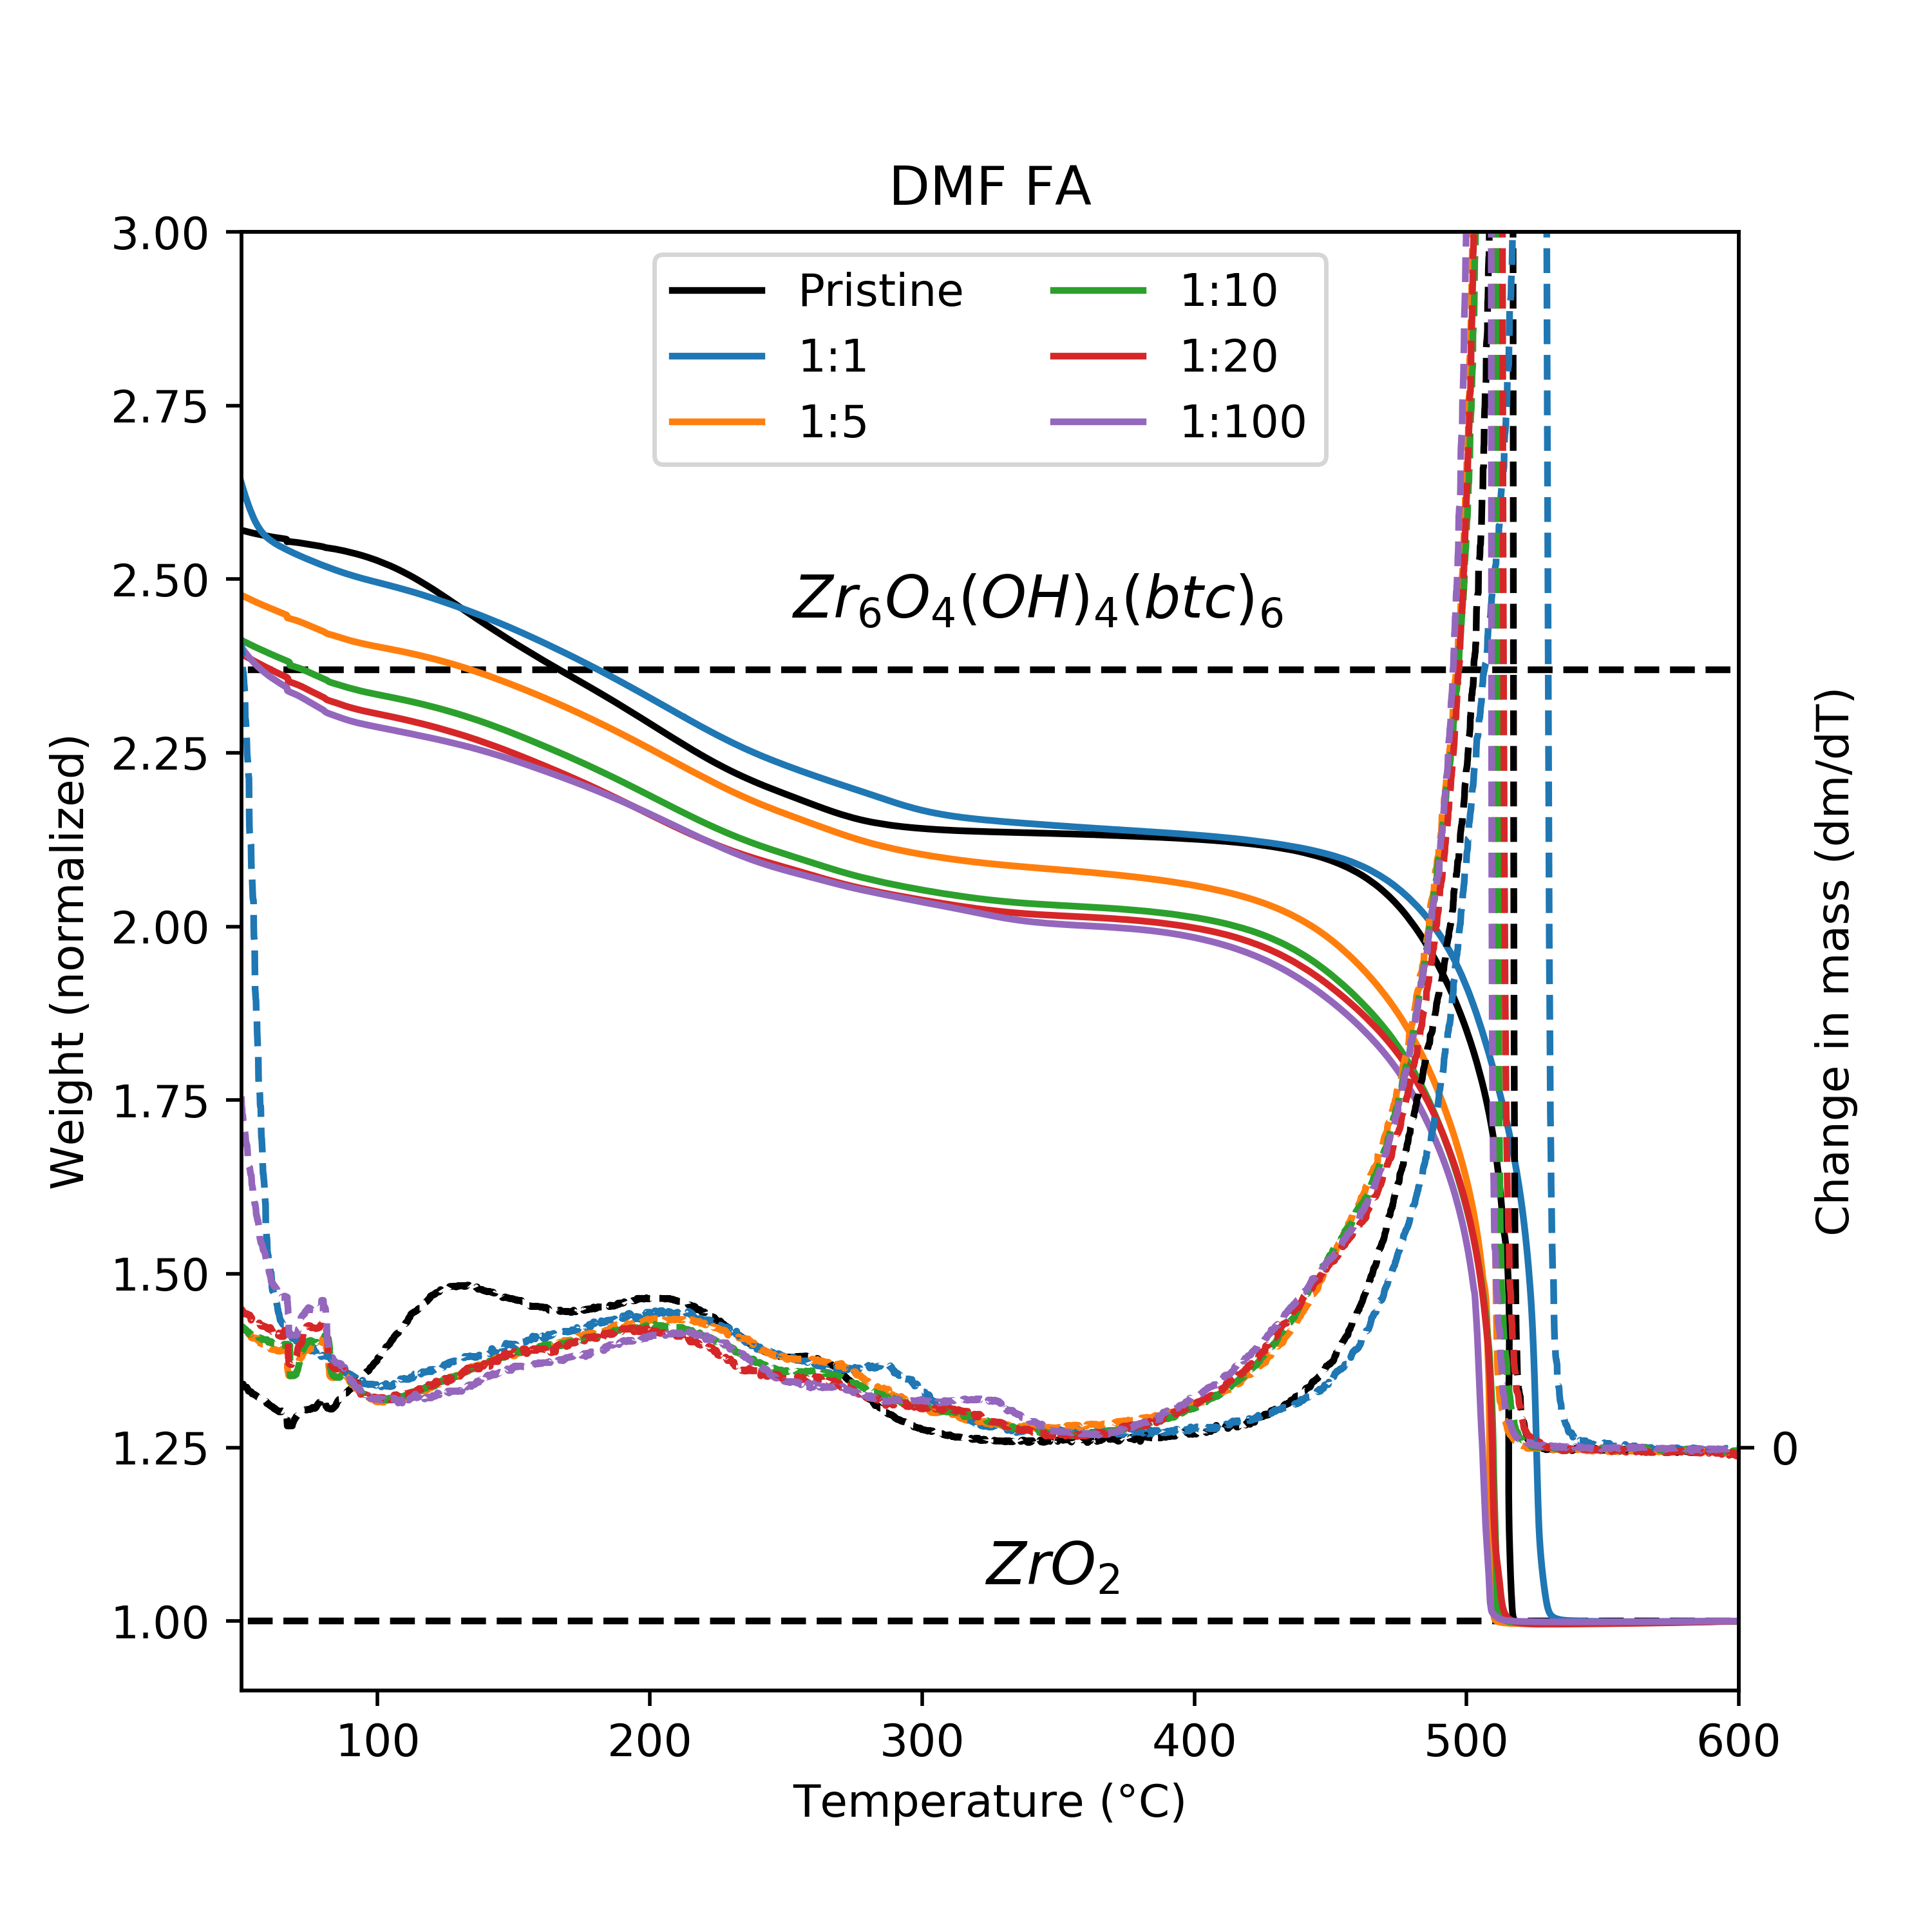
\includegraphics[width=\textwidth]{tga/DMF-FA}%
        \label{appx:def:fgr:tga-dmf-fa}
    \end{subfigure}
    \begin{subfigure}{0.45\linewidth}
        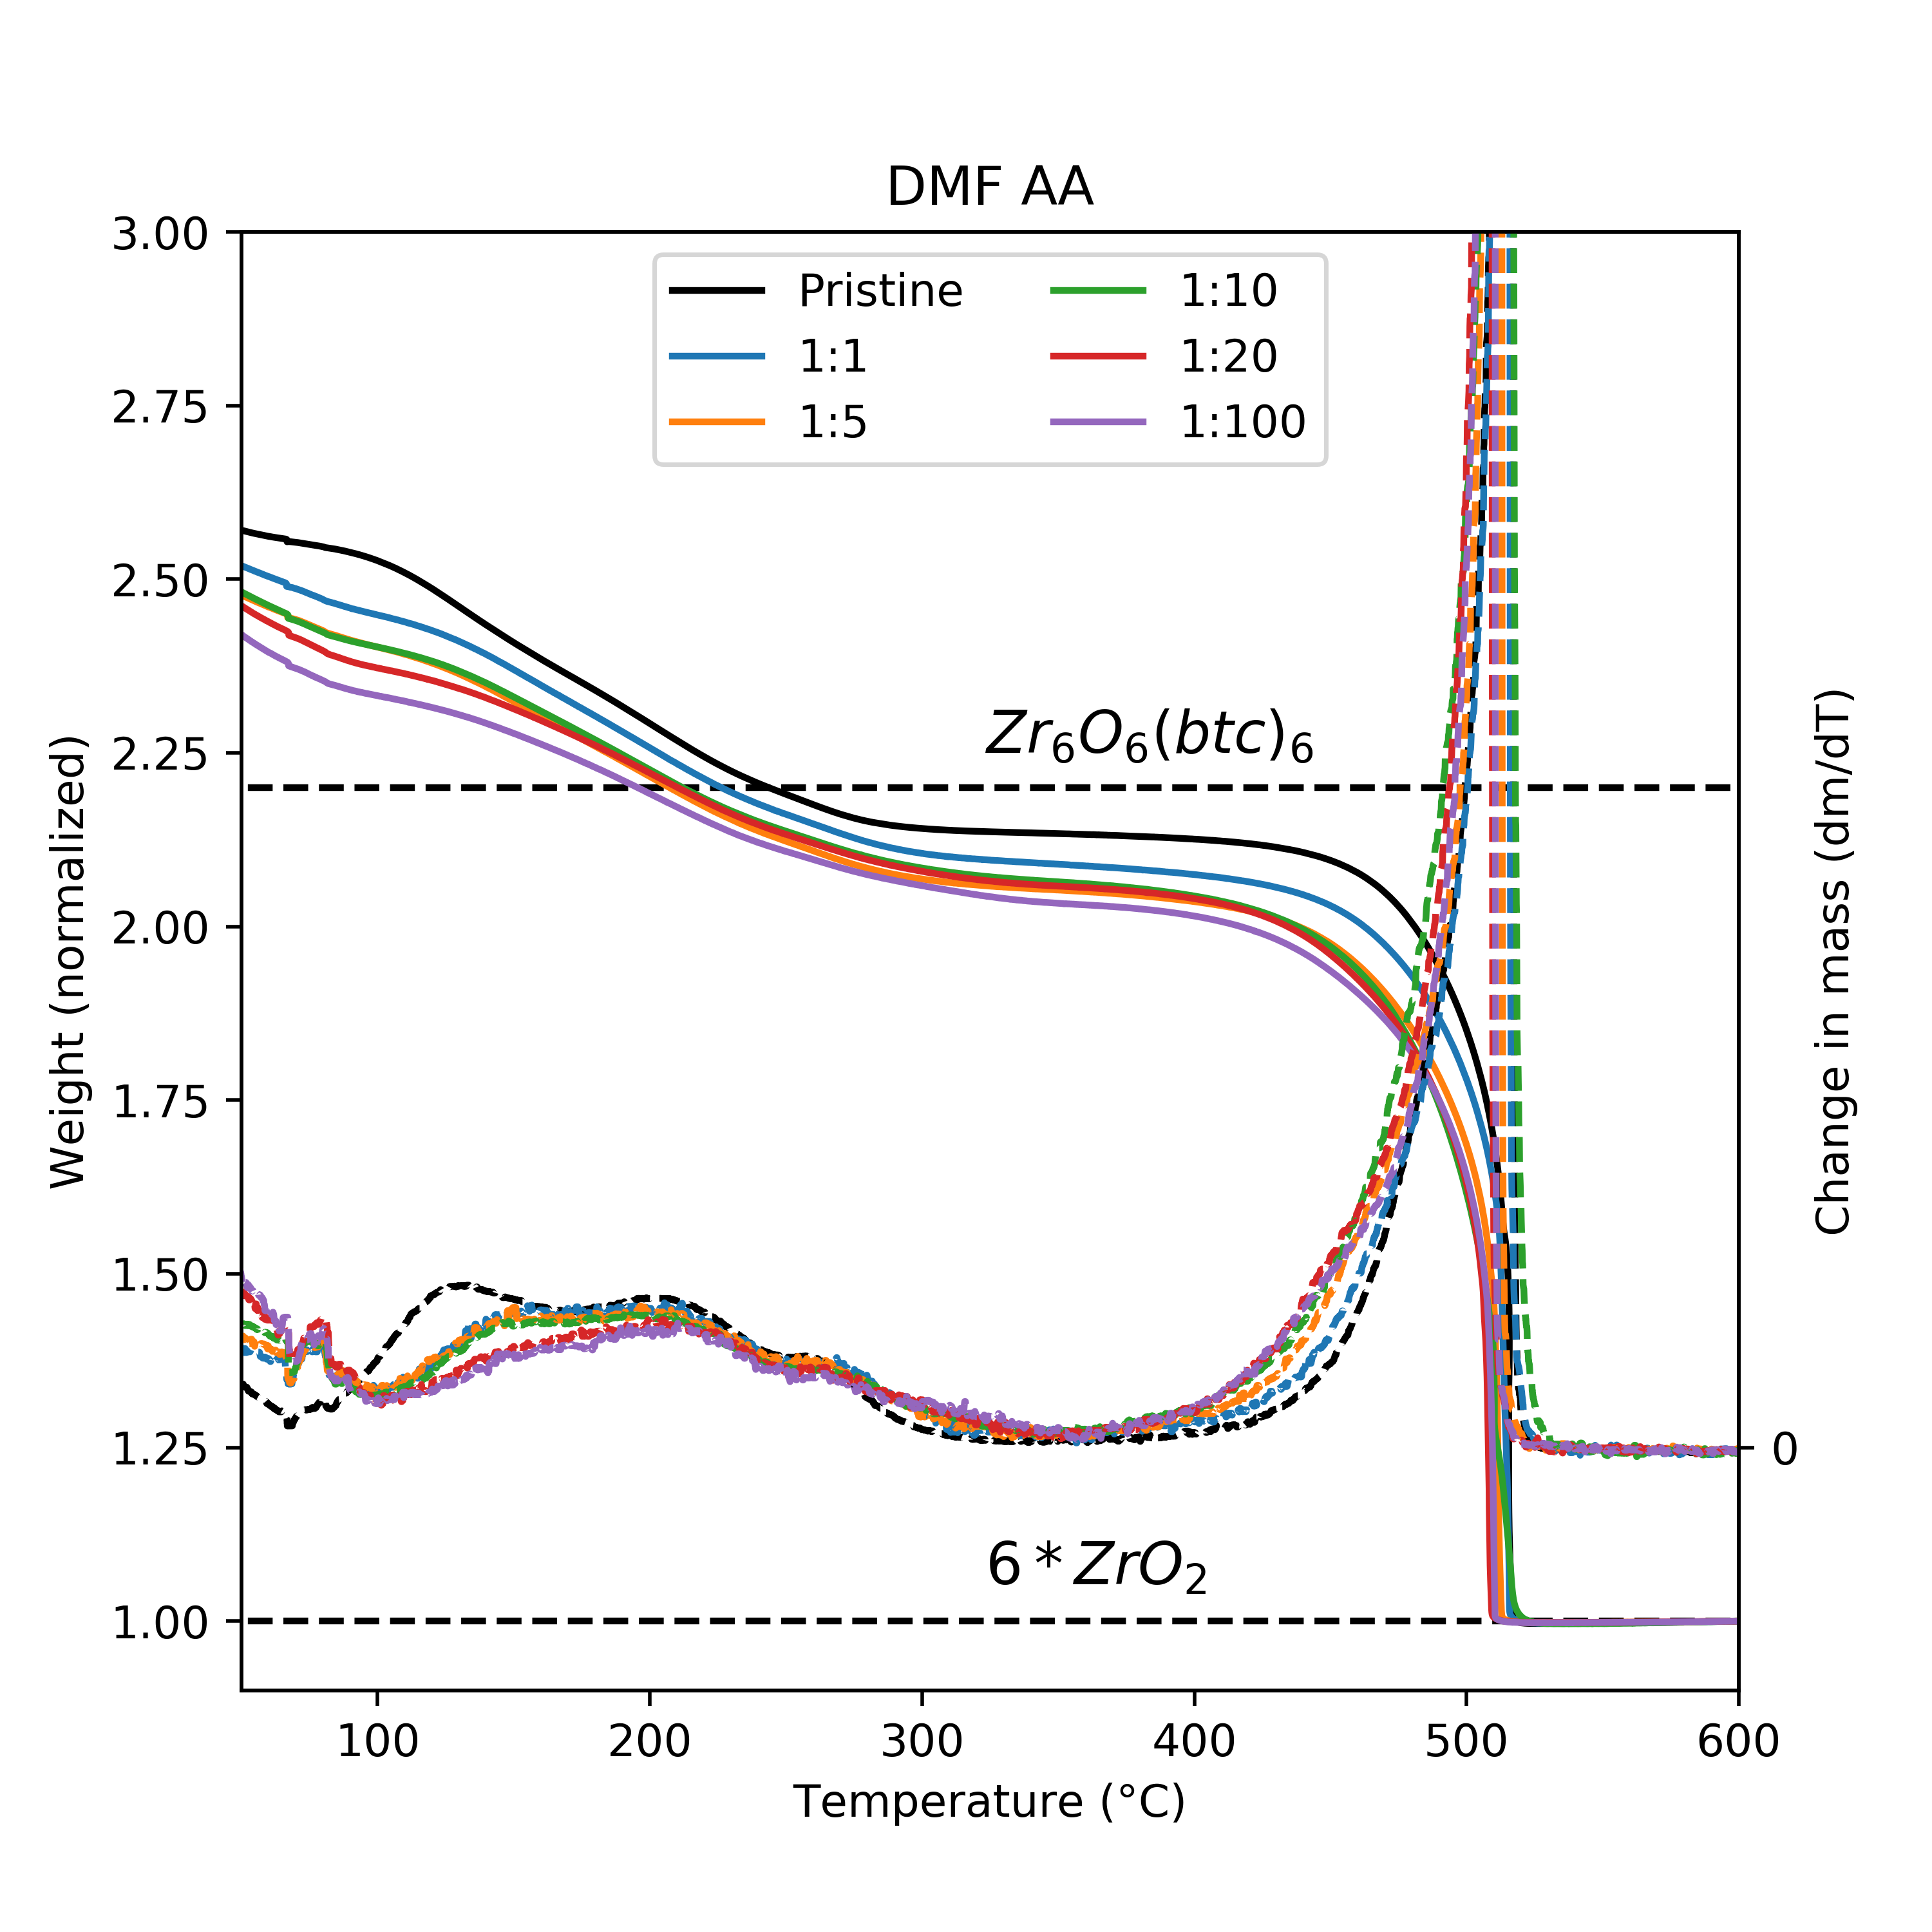
\includegraphics[width=\textwidth]{tga/DMF-AA}%
        \label{appx:def:fgr:tga-dmf-aa}
    \end{subfigure}

    
    \begin{subfigure}{0.45\linewidth}
        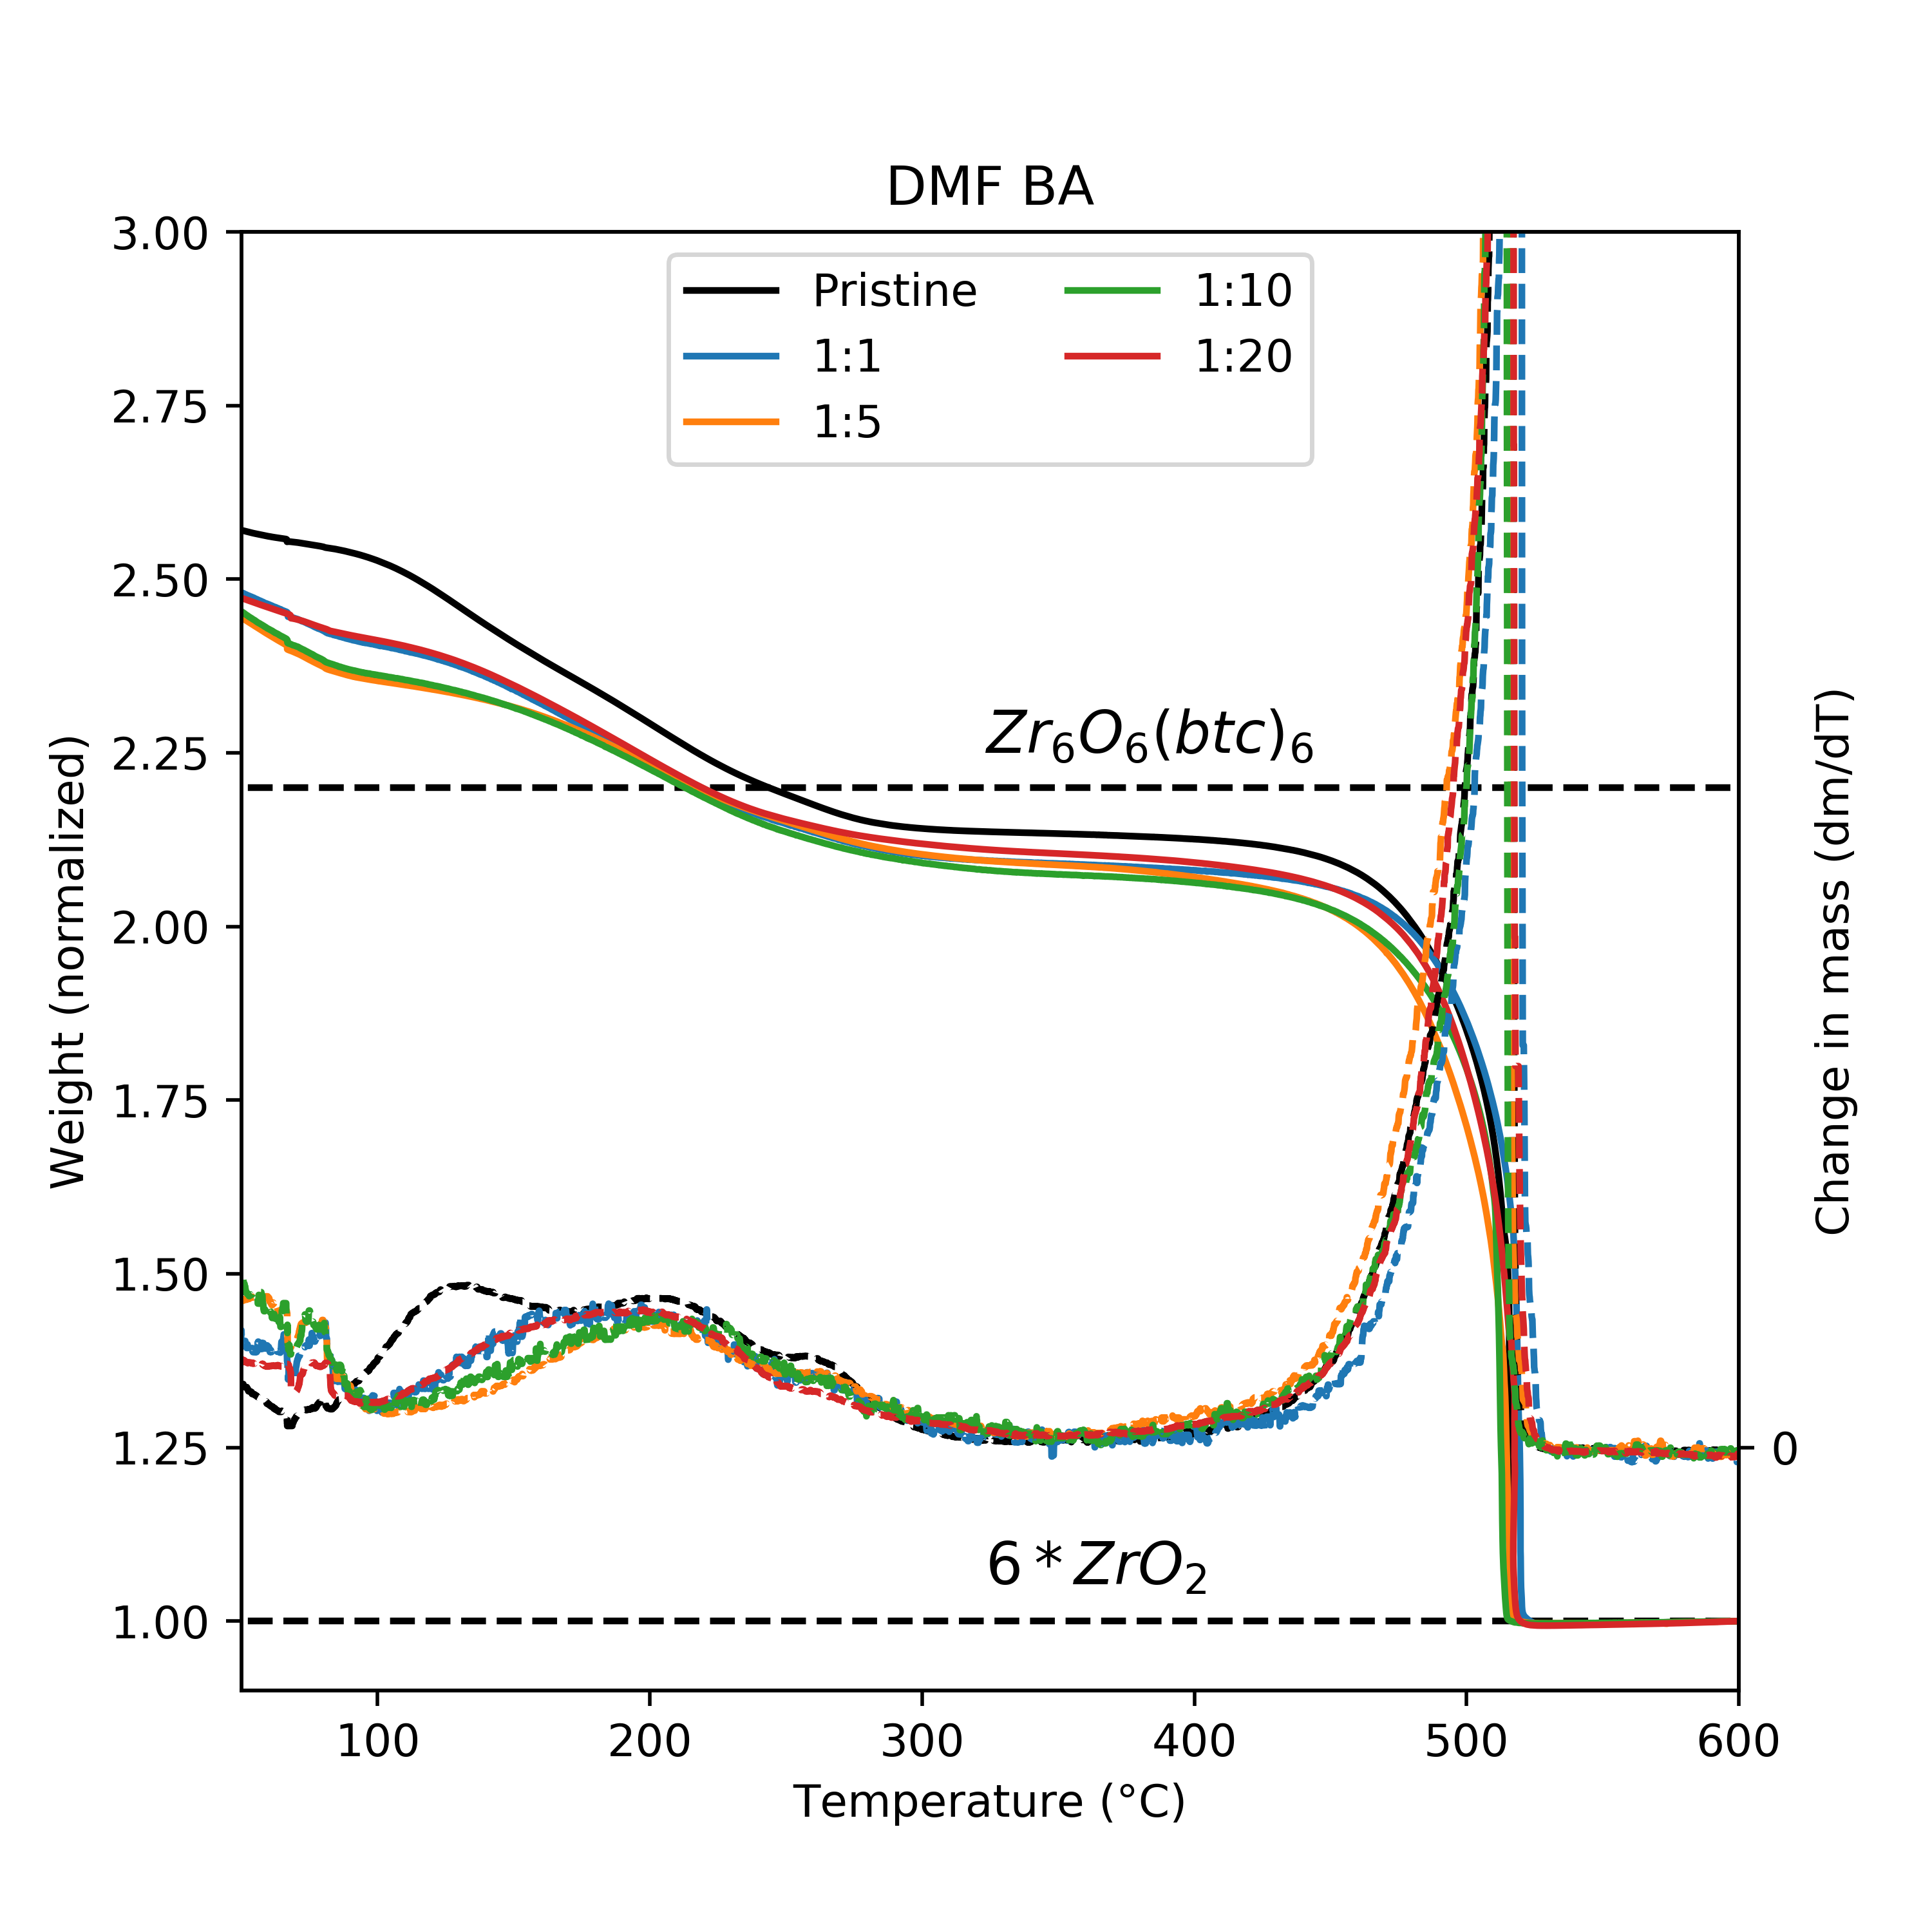
\includegraphics[width=\textwidth]{tga/DMF-BA}%
        \label{appx:def:fgr:tga-dmf-ba}
    \end{subfigure}

    \caption{TGA curves}%
    \label{appx:def:fgr:tga-dataset}
\end{figure}
\begin{figure}[htb]\ContinuedFloat{}
    \centering

    \begin{subfigure}{0.45\linewidth}
        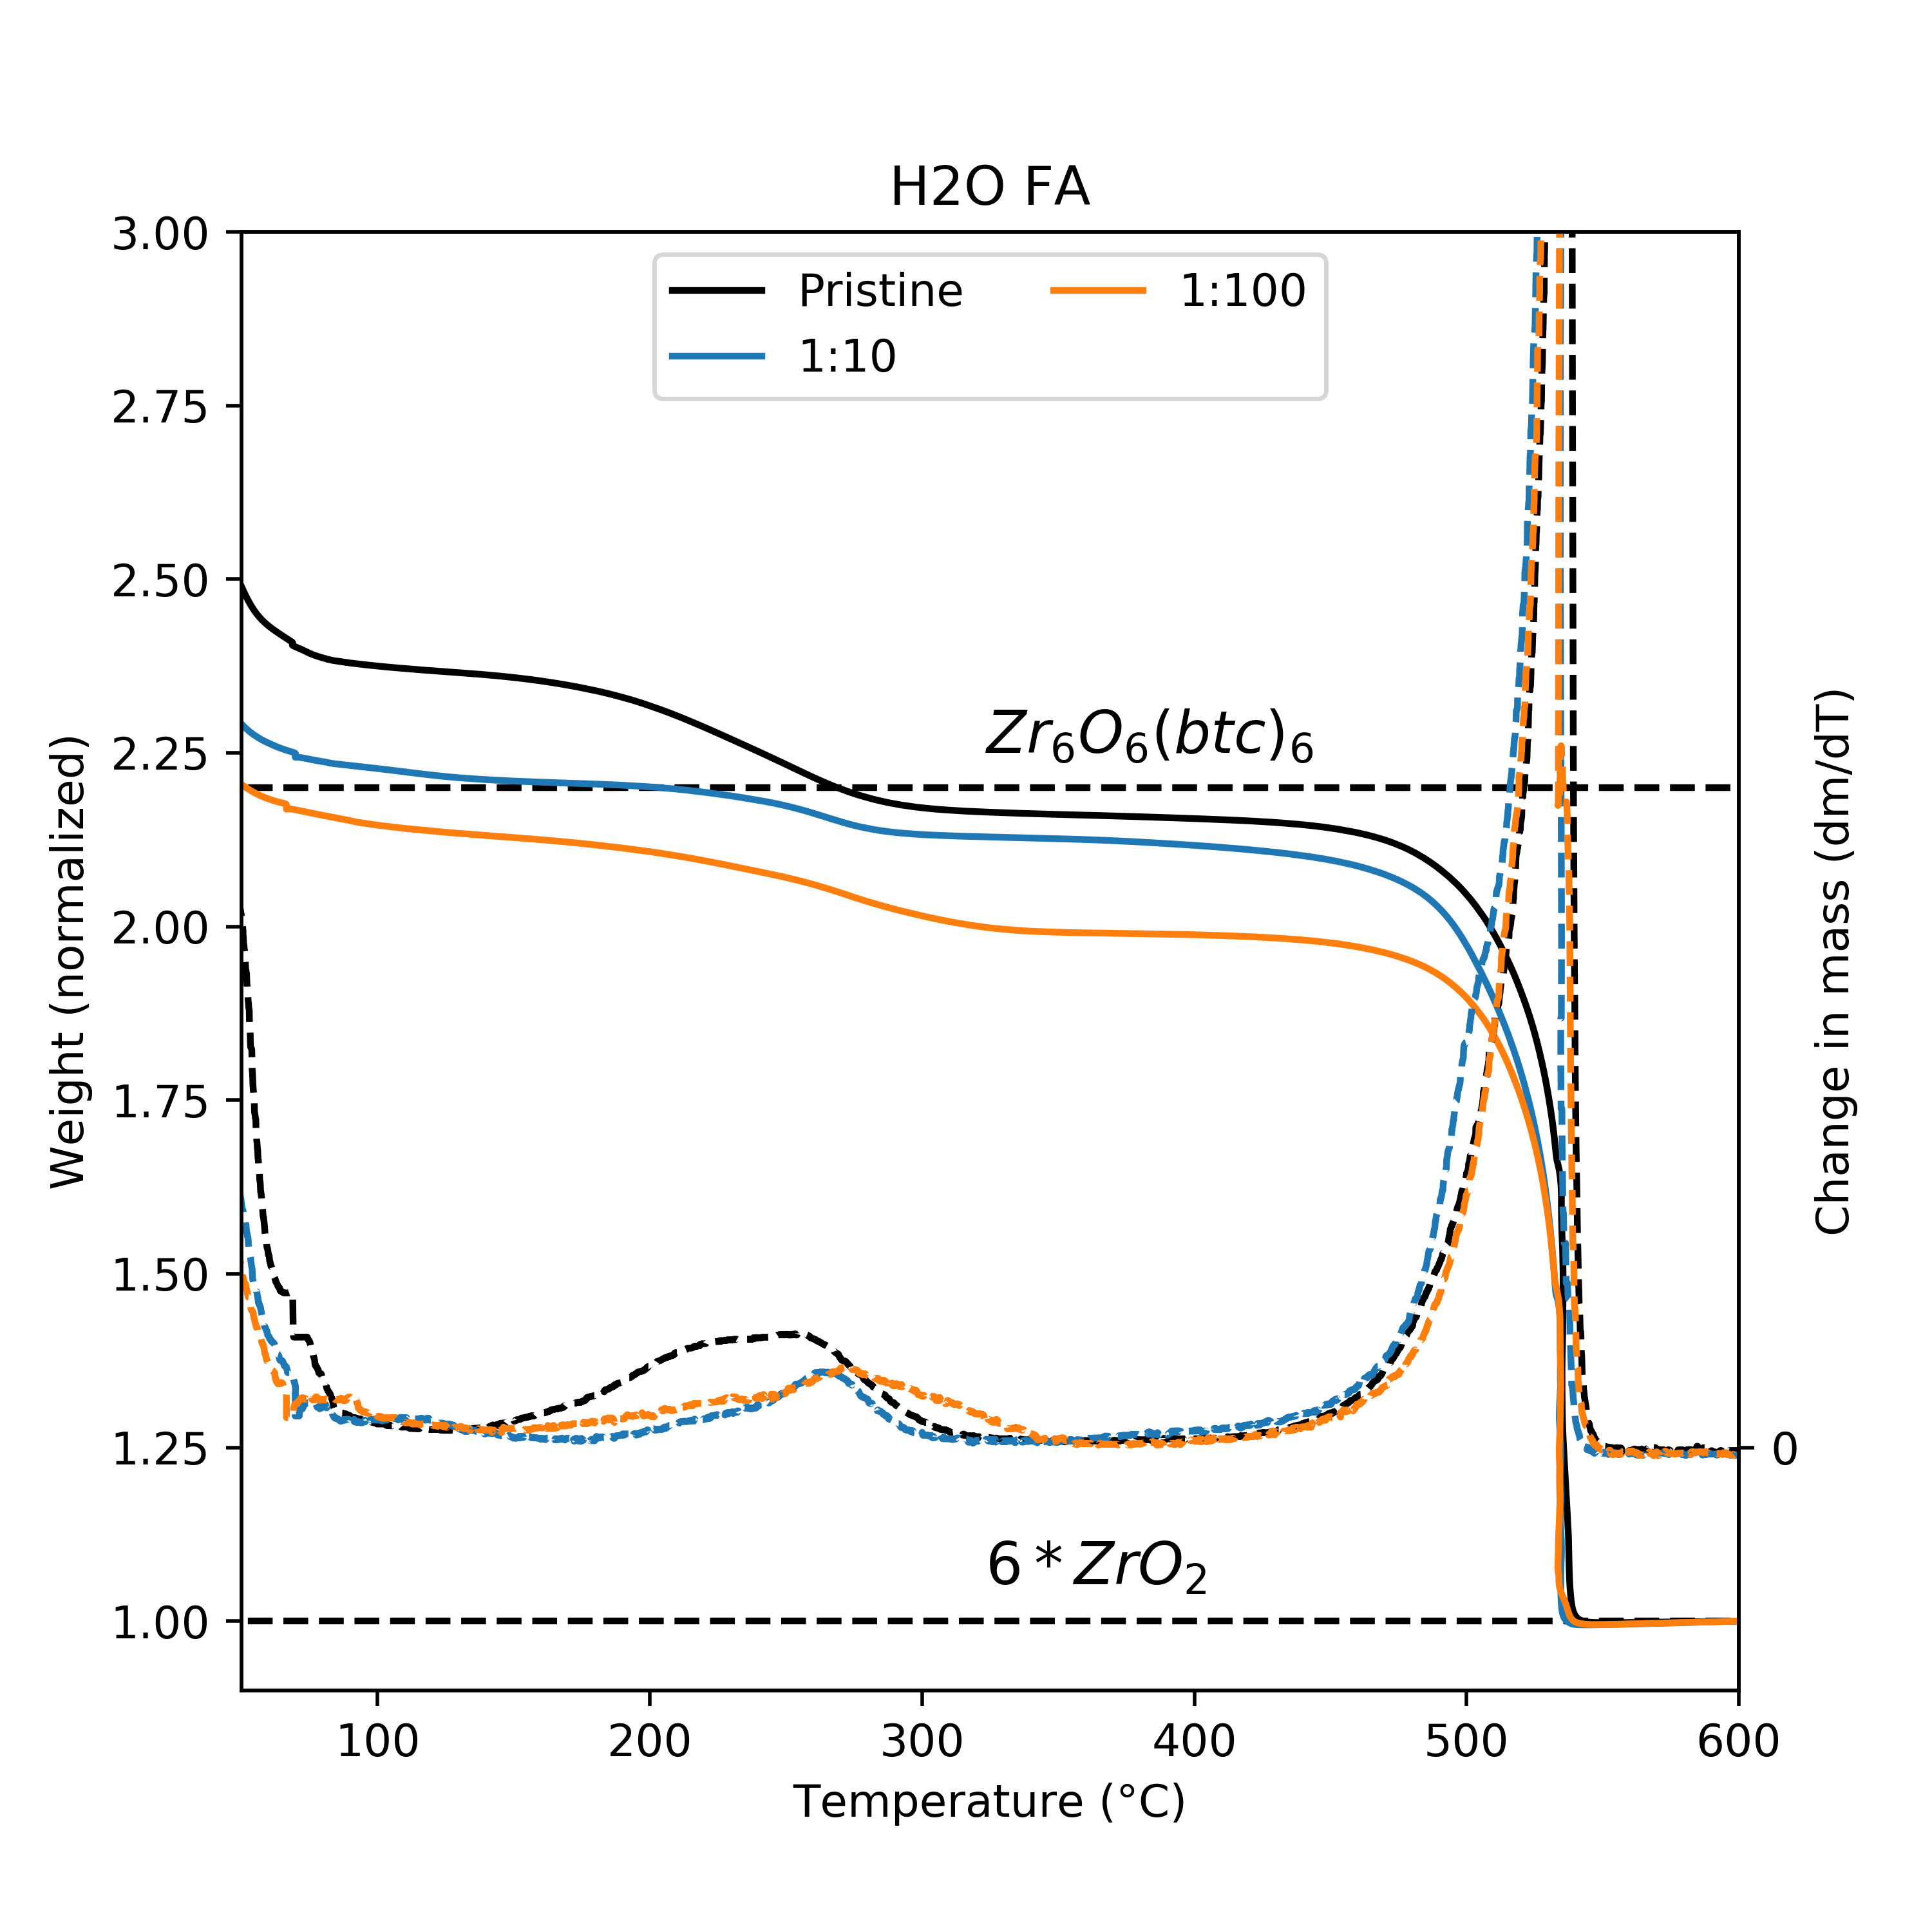
\includegraphics[width=\textwidth]{tga/H2O-FA}%
        \label{appx:def:fgr:tga-h2o-fa}
    \end{subfigure}
    \begin{subfigure}{0.45\linewidth}
        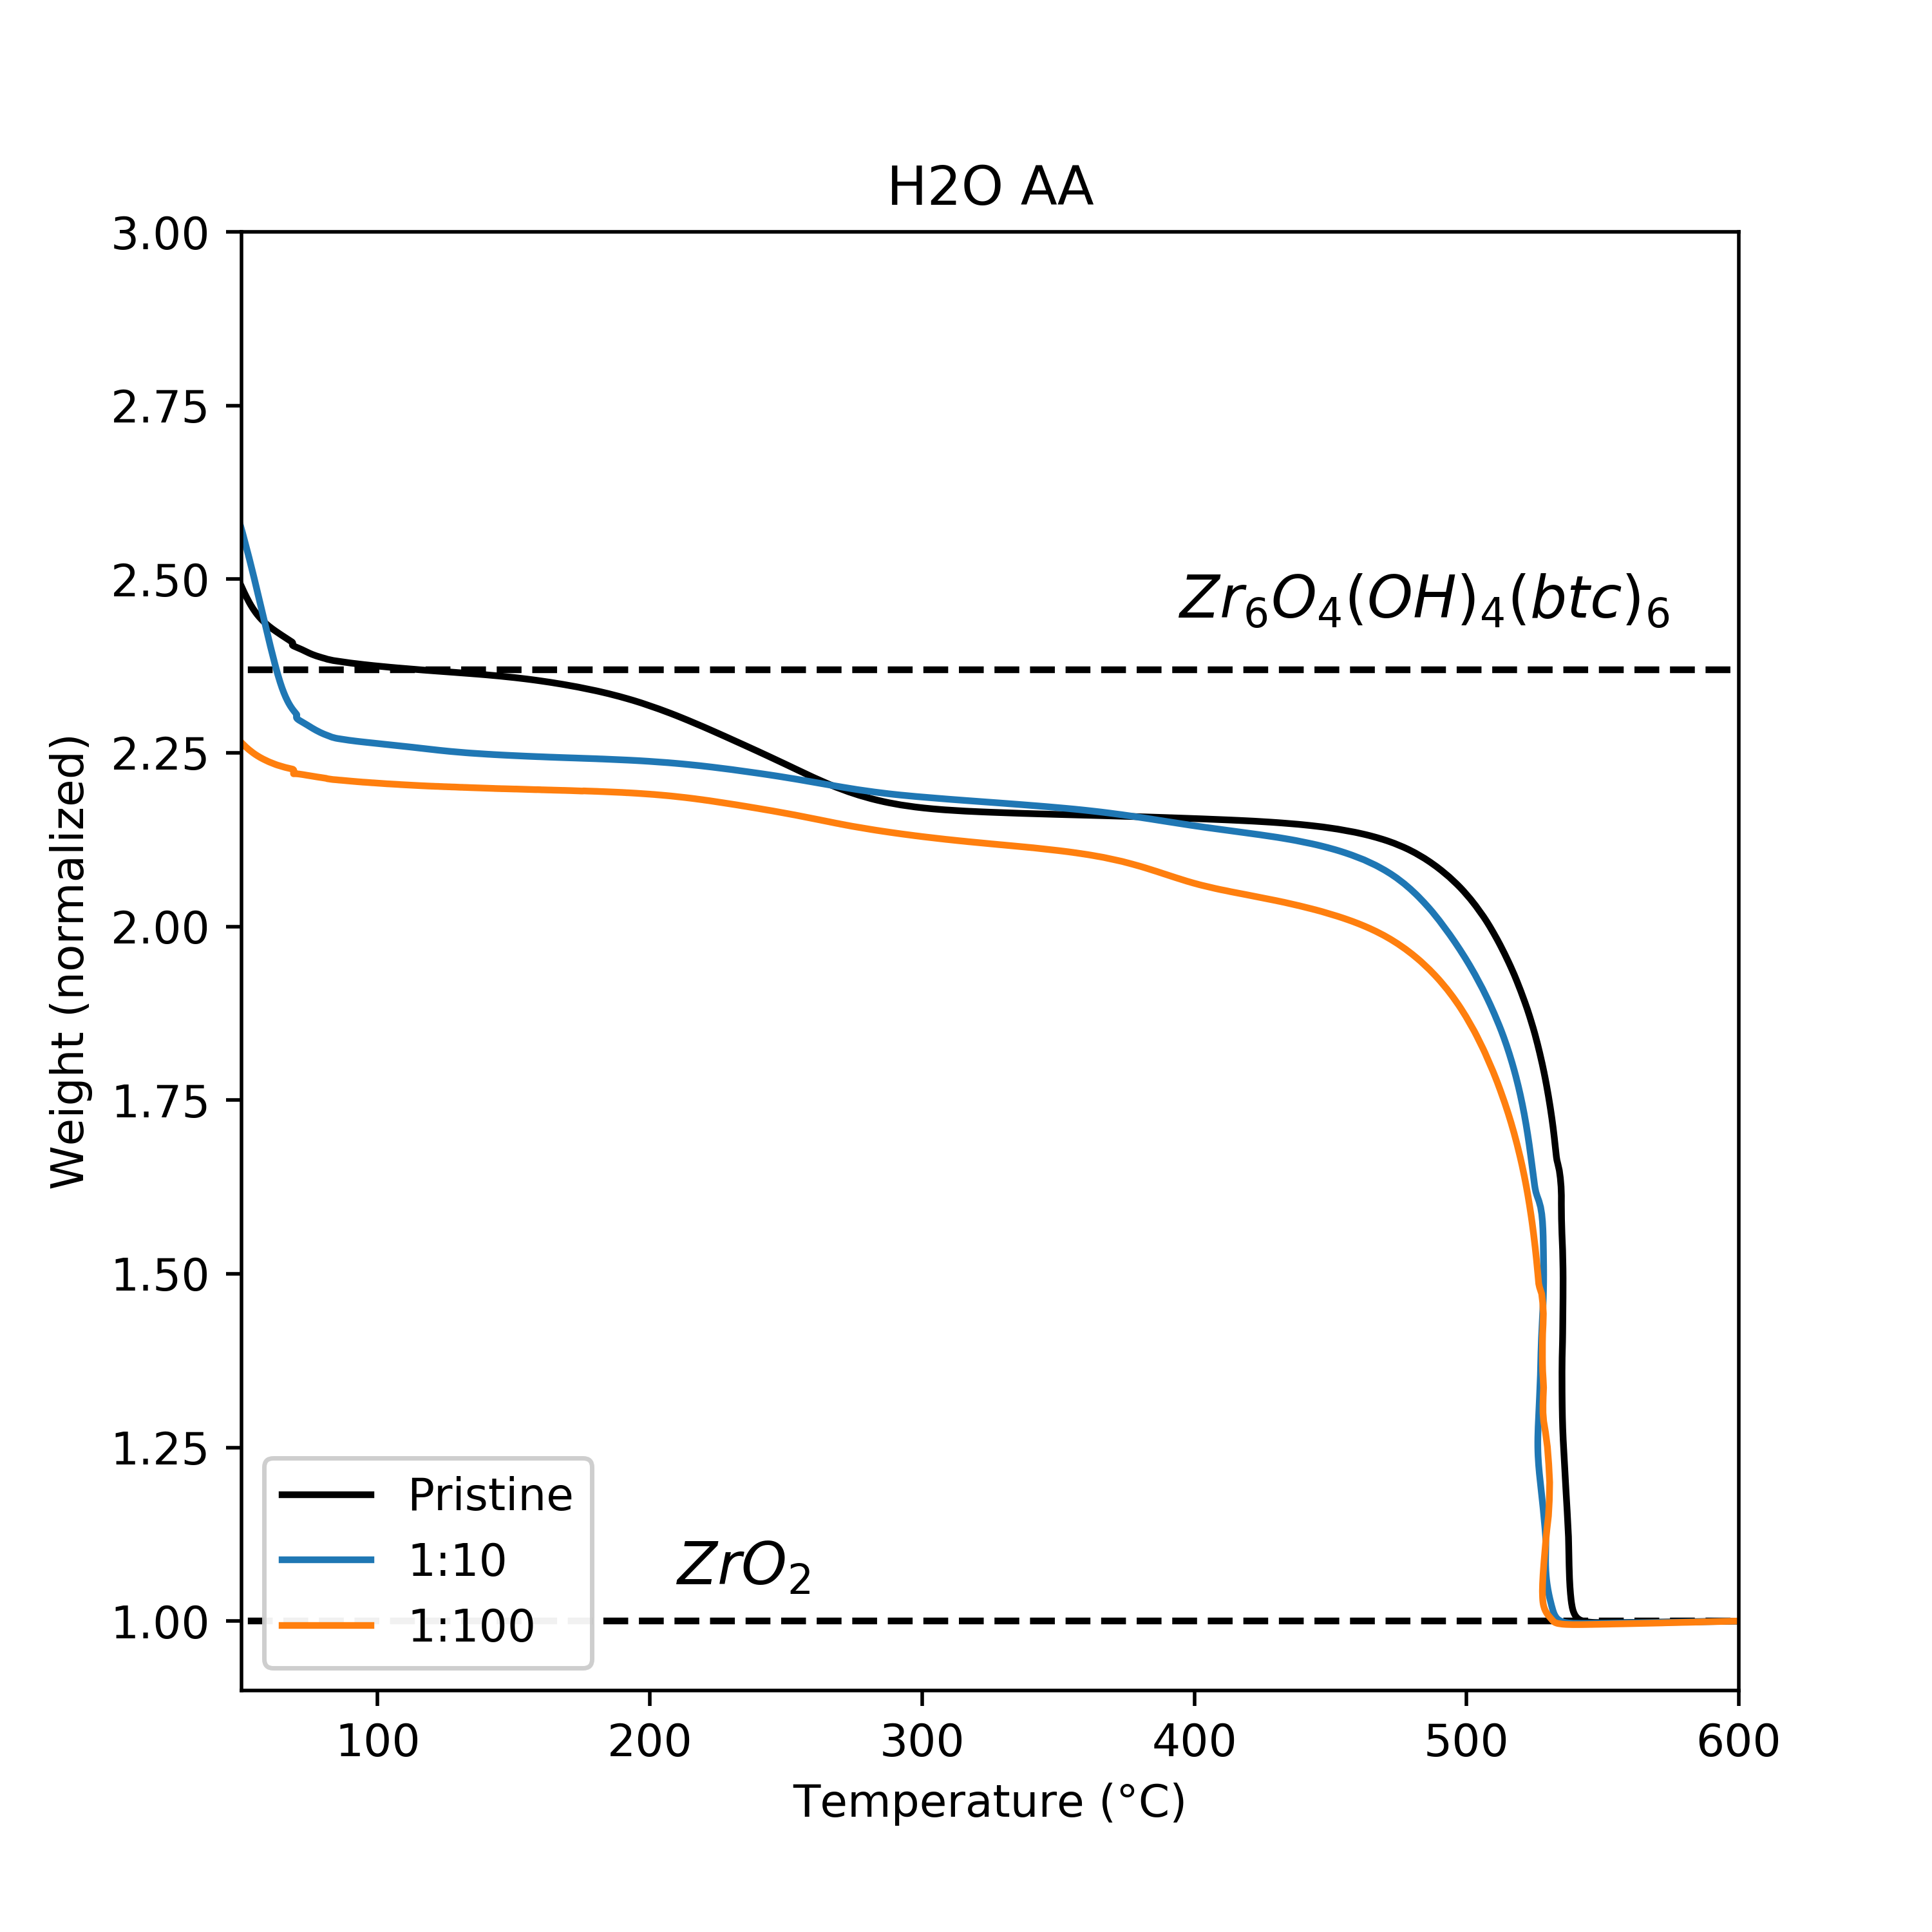
\includegraphics[width=\textwidth]{tga/H2O-AA}%
        \label{appx:def:fgr:tga-h2o-aa}
    \end{subfigure}

    \begin{subfigure}{0.45\linewidth}
        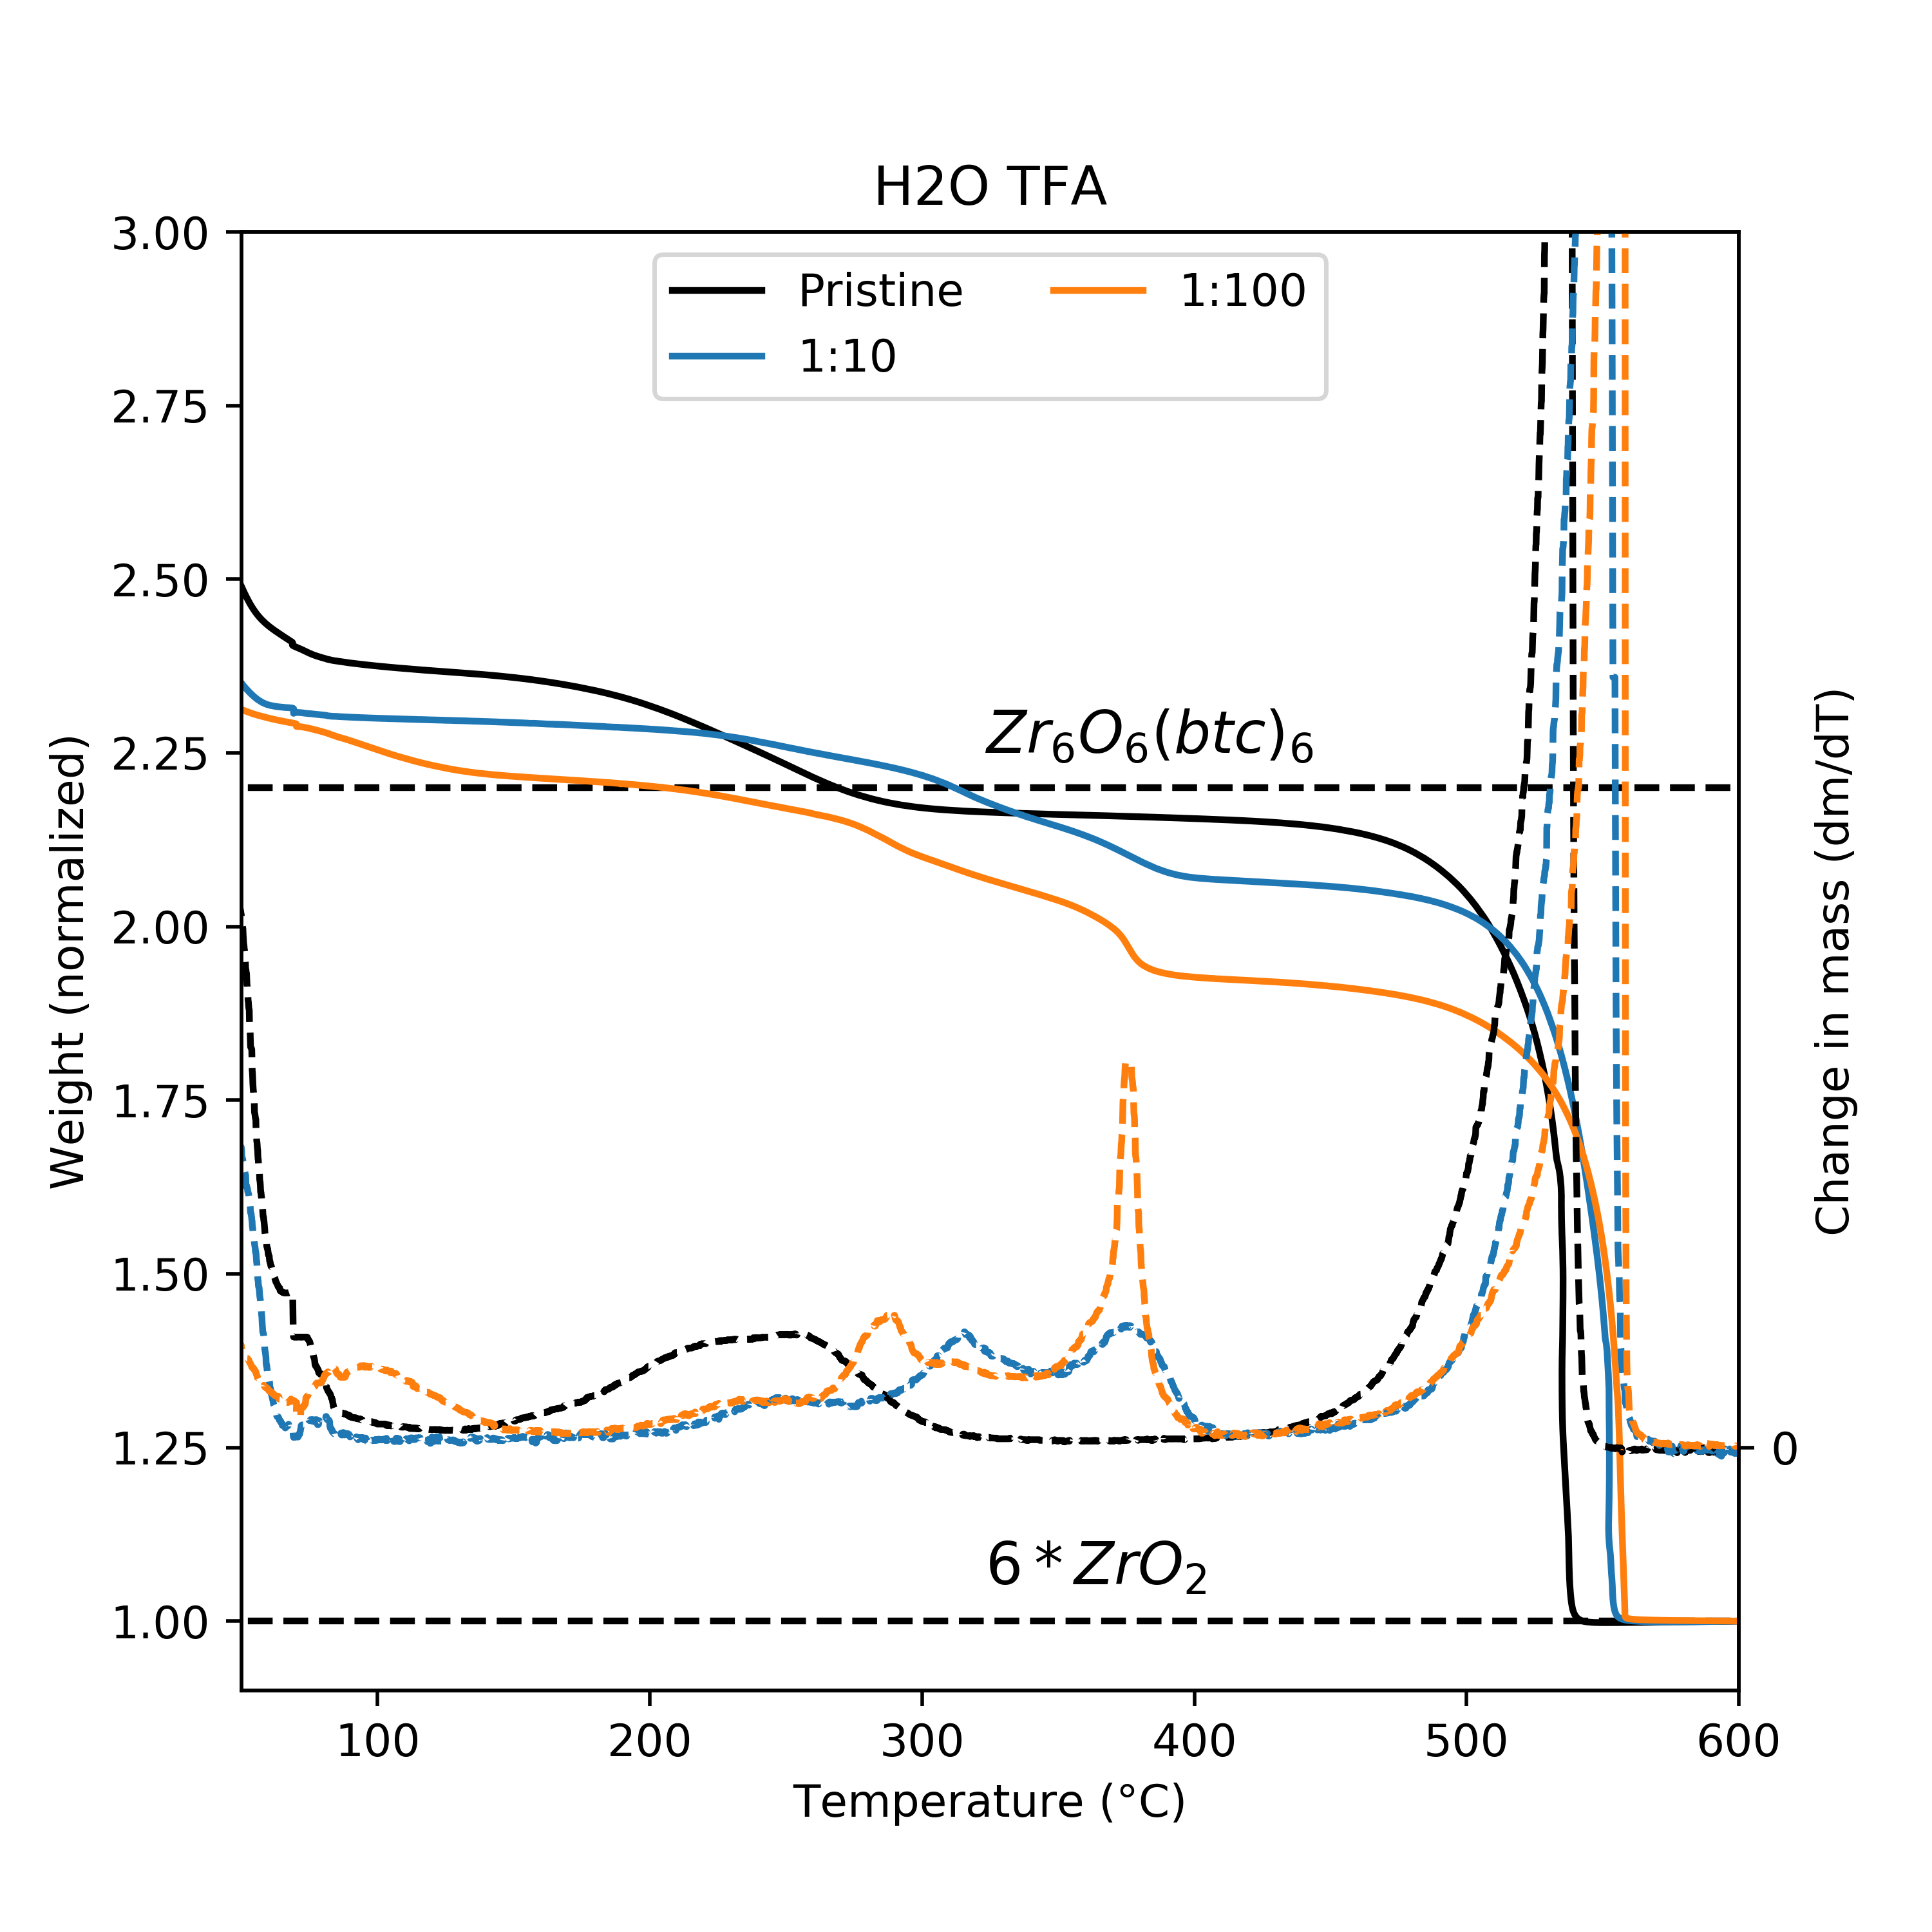
\includegraphics[width=\textwidth]{tga/H2O-TFA}%
        \label{appx:def:fgr:tga-h2o-tfa}
    \end{subfigure}

    \caption{TGA curves}%
\end{figure}
\begin{figure}[htb]\ContinuedFloat{}
    \centering

    \begin{subfigure}{0.45\linewidth}
        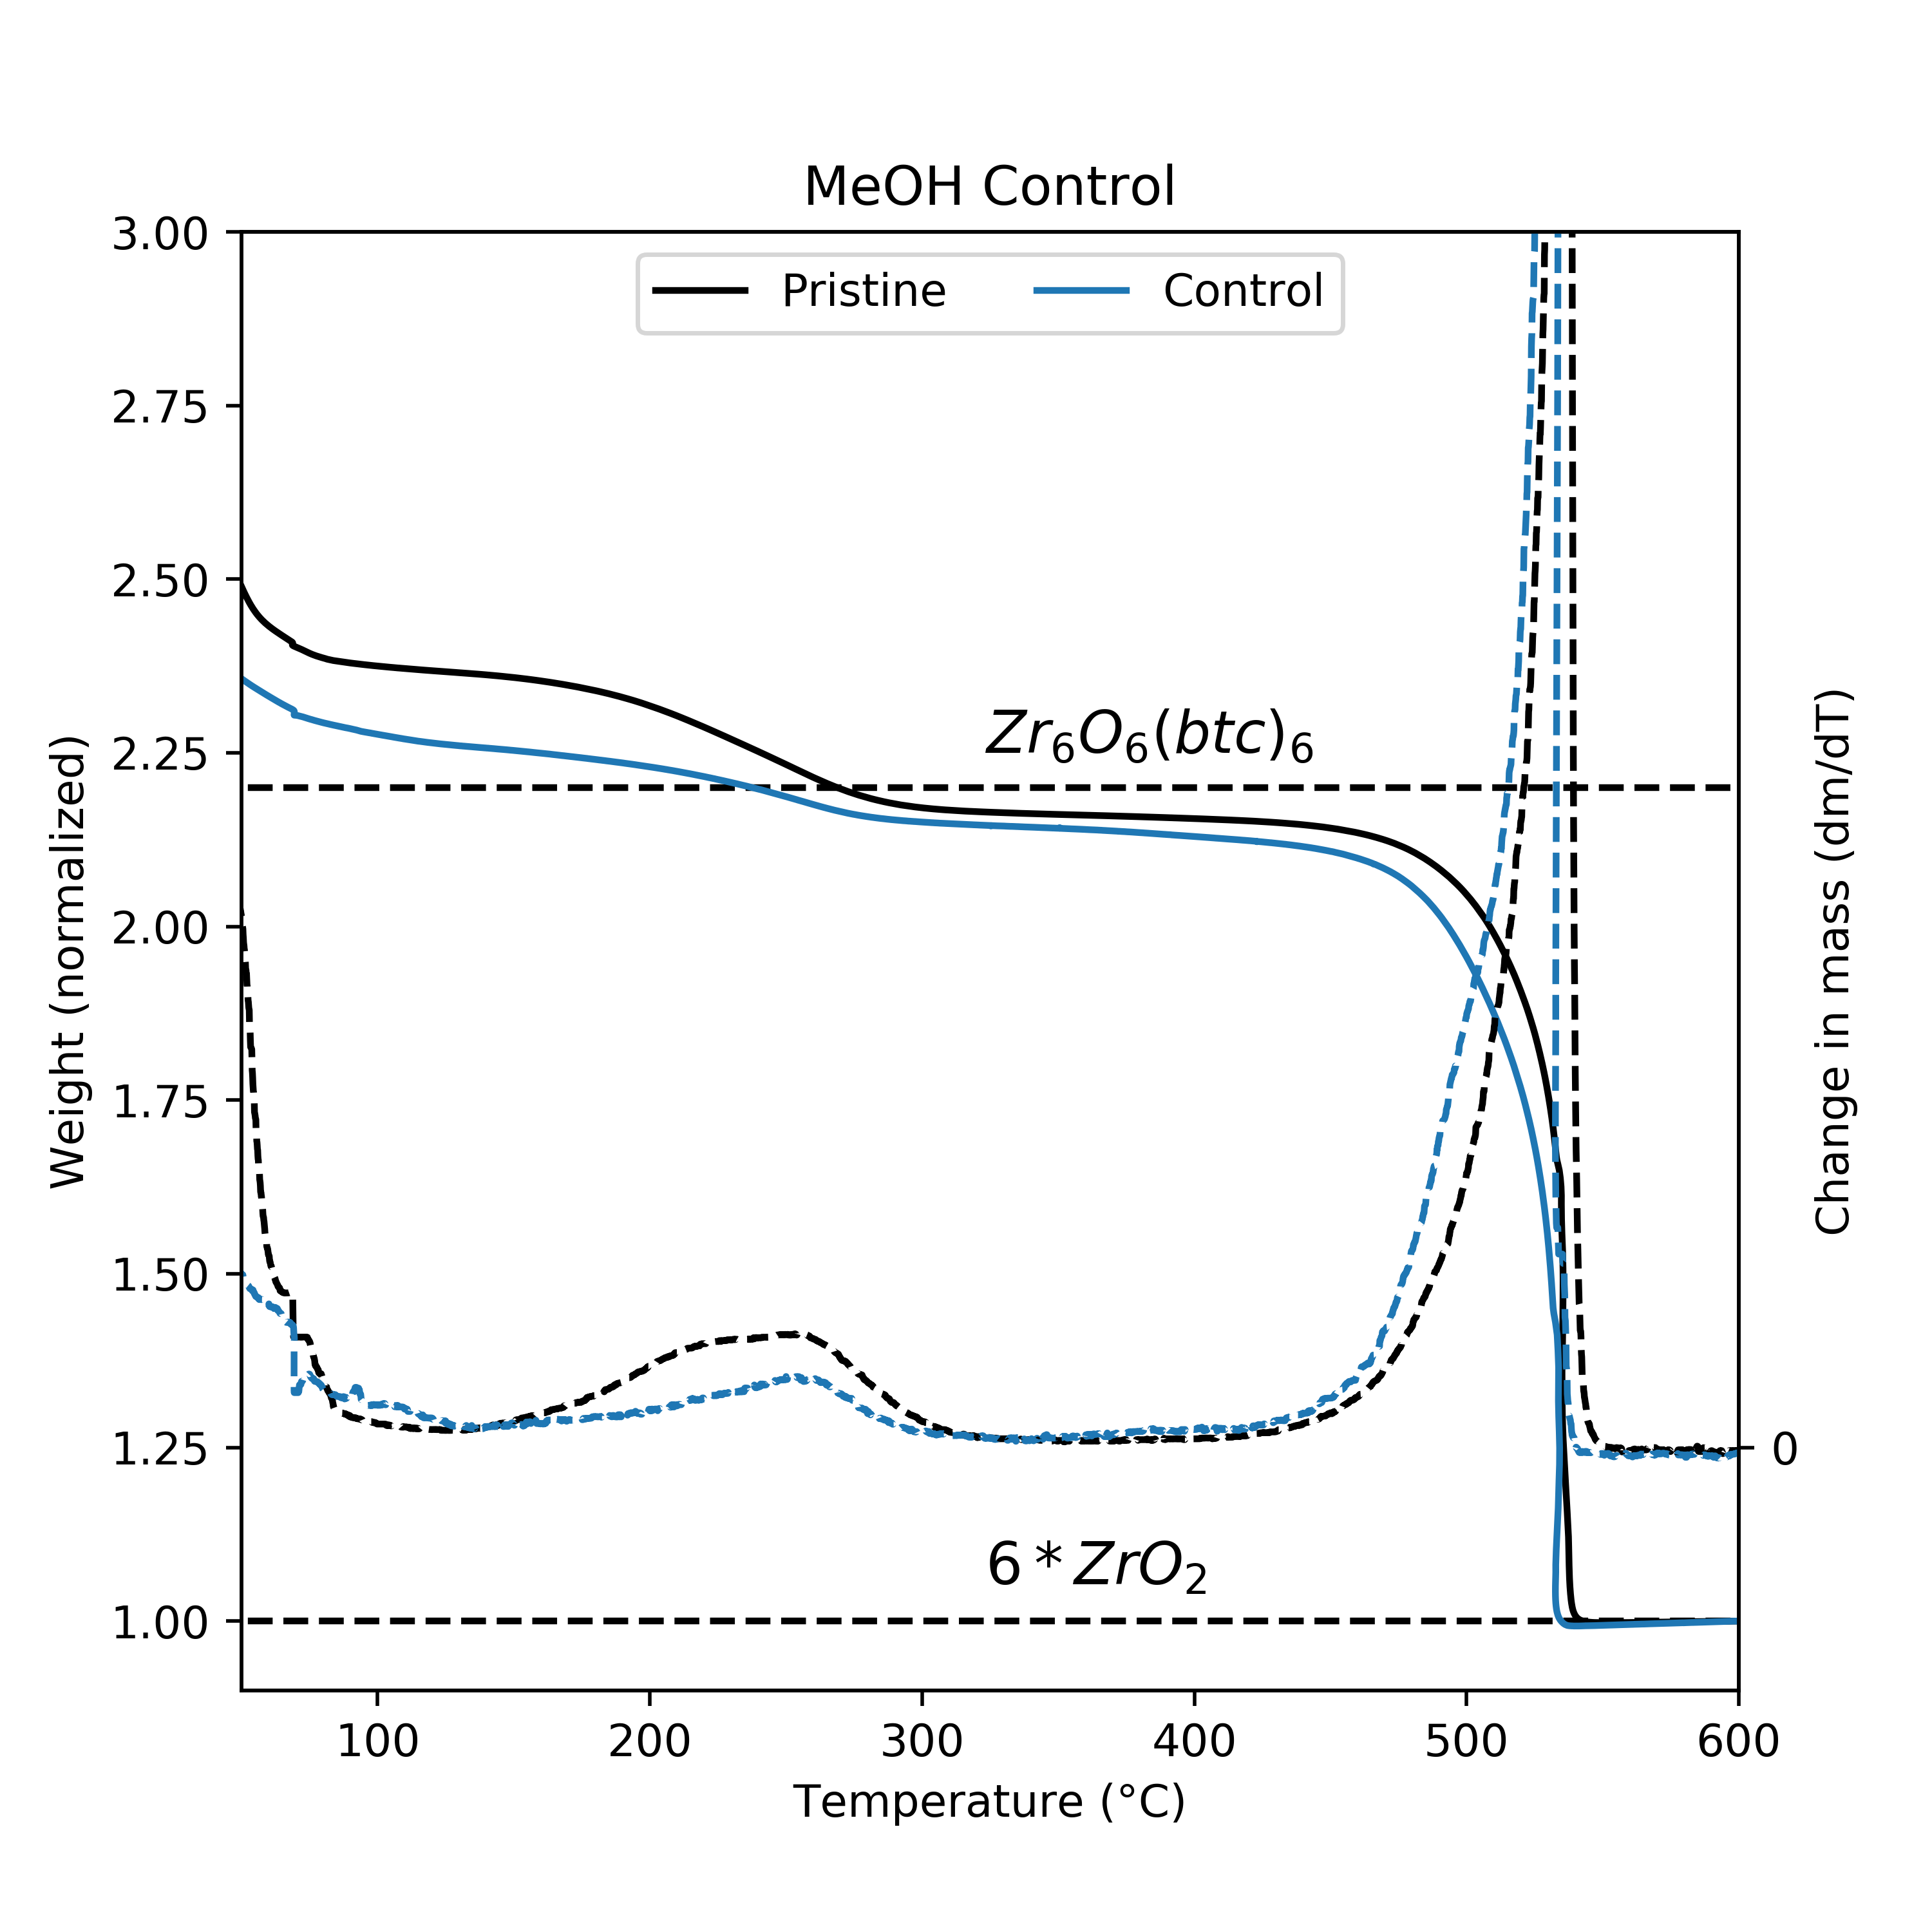
\includegraphics[width=\textwidth]{tga/MeOH-Control}%
        \label{appx:def:fgr:tga-meoh-cont}
    \end{subfigure}

    \begin{subfigure}{0.45\linewidth}
        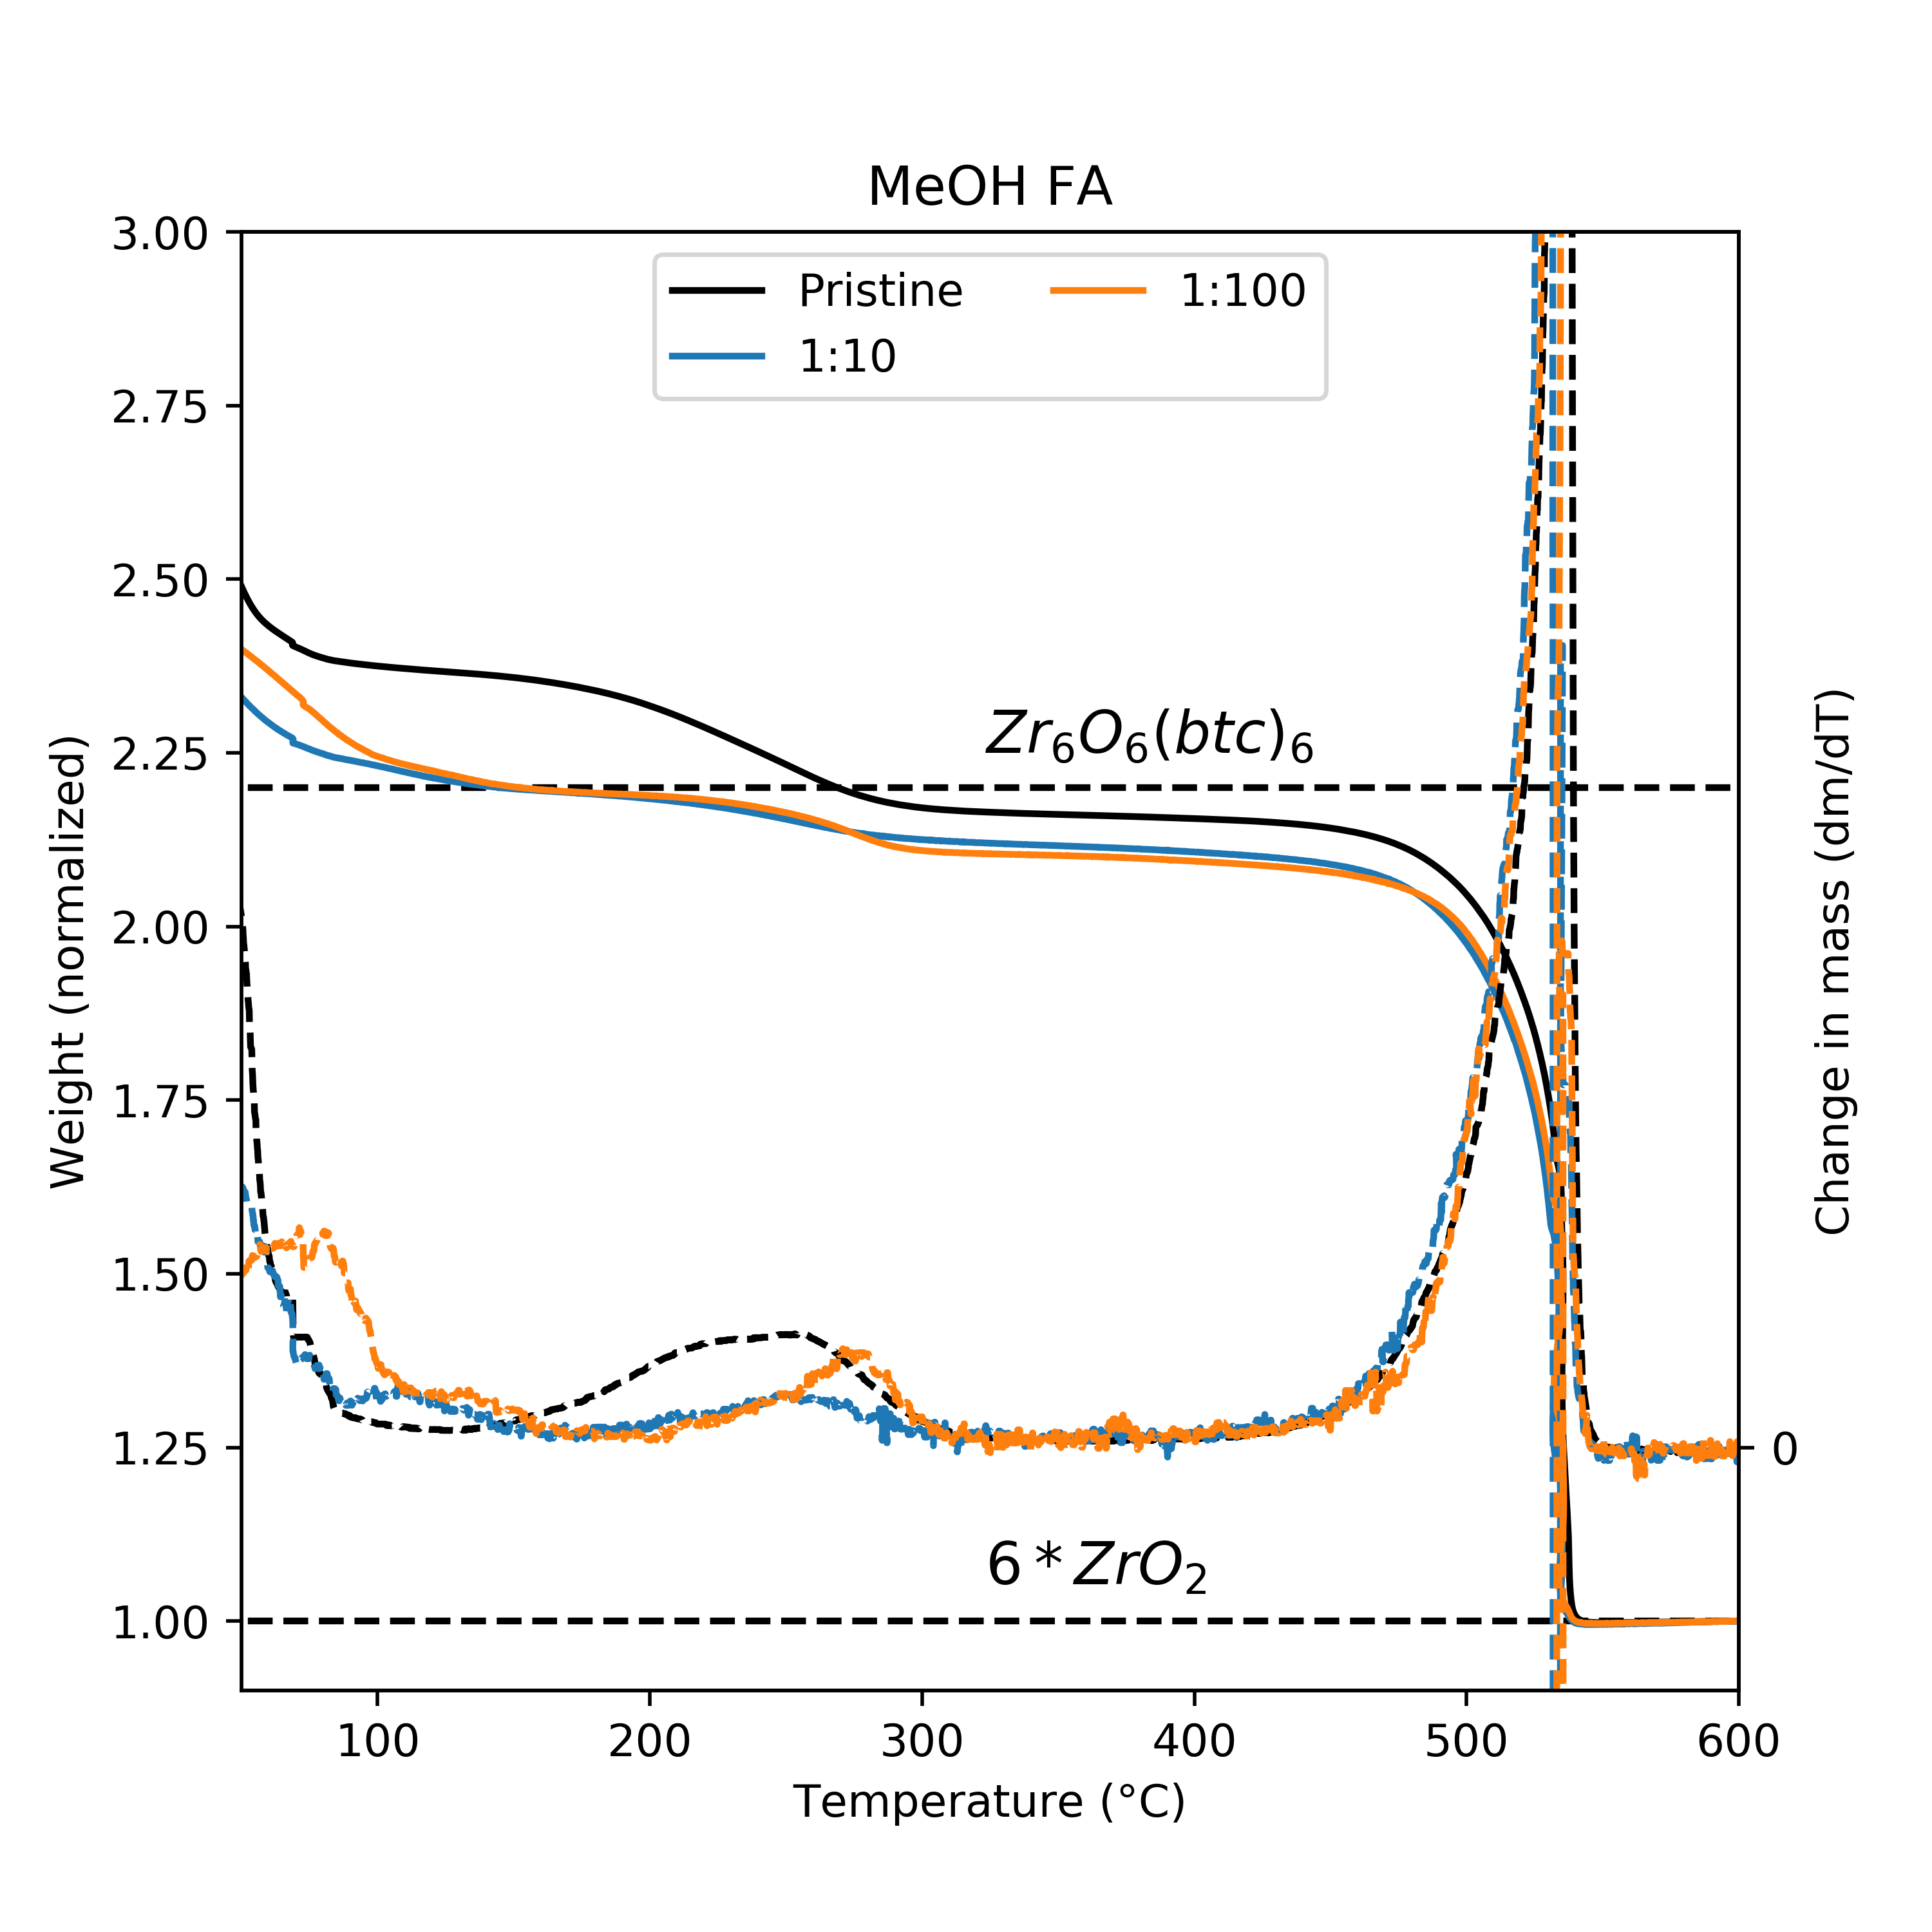
\includegraphics[width=\textwidth]{tga/MeOH-FA}%
        \label{appx:def:fgr:tga-meoh-fa}
    \end{subfigure}
    \begin{subfigure}{0.45\linewidth}
        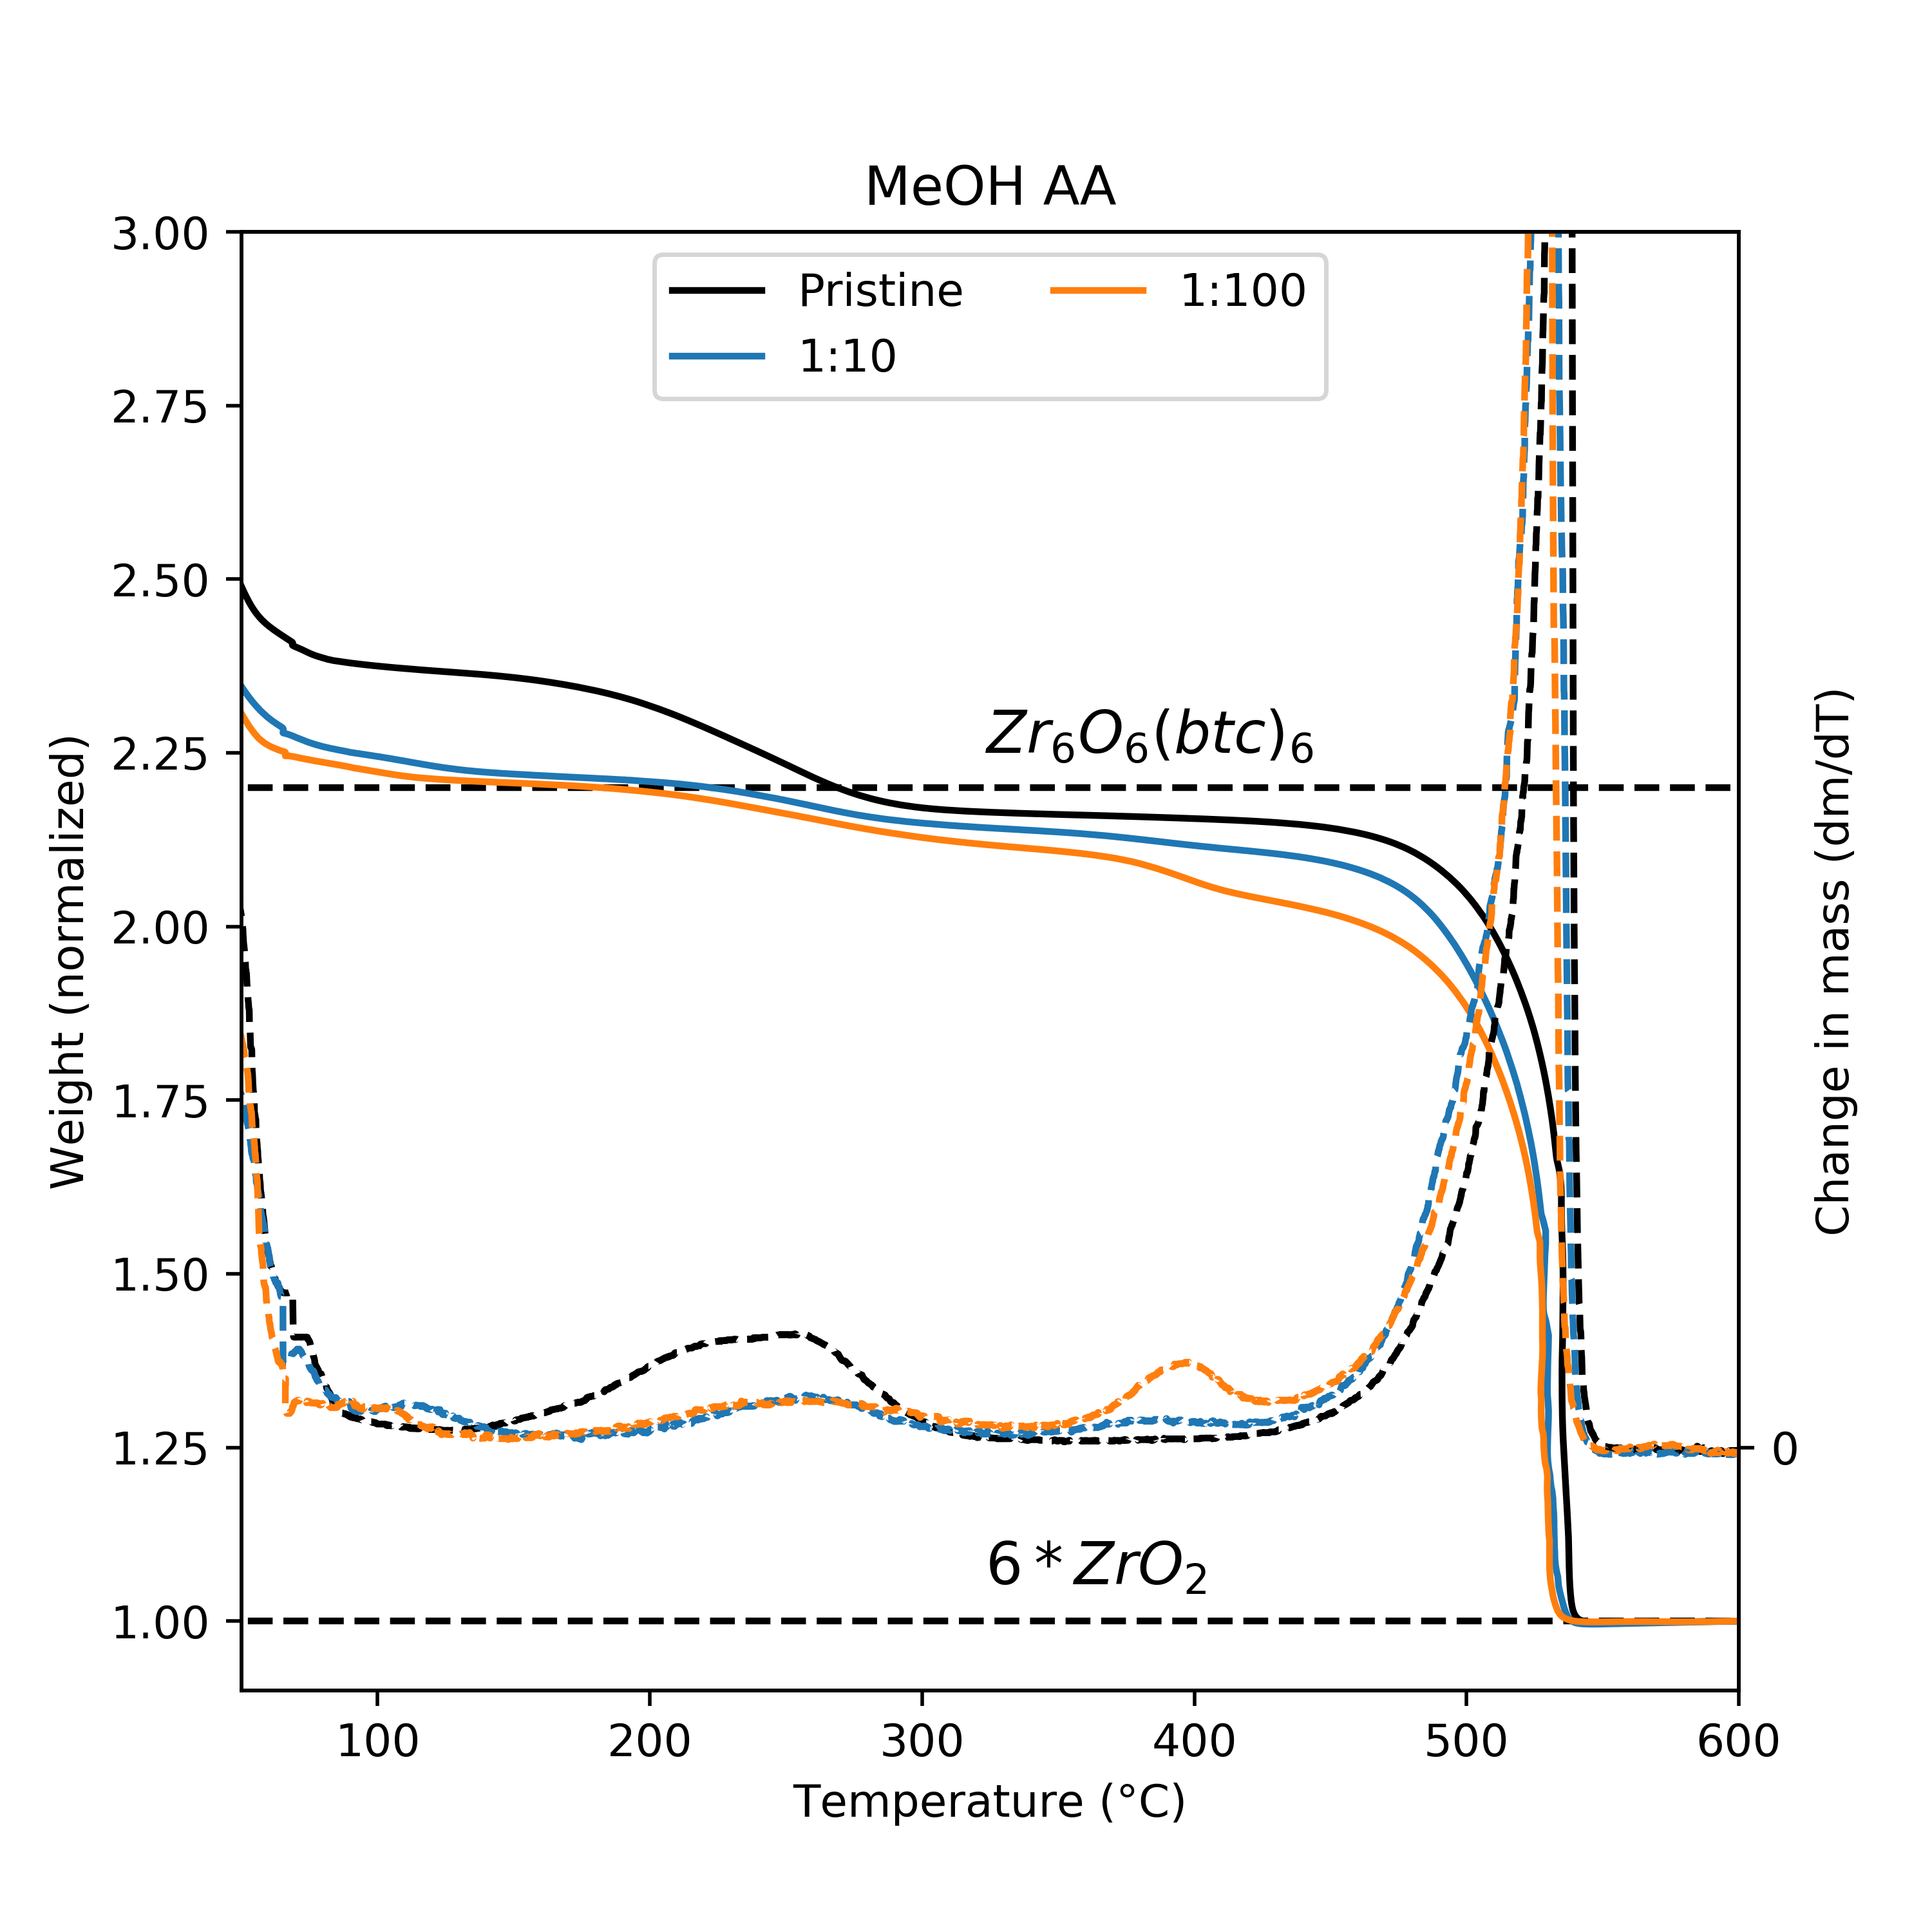
\includegraphics[width=\textwidth]{tga/MeOH-AA}%
        \label{appx:def:fgr:tga-meoh-aa}
    \end{subfigure}
    
    \begin{subfigure}{0.45\linewidth}
        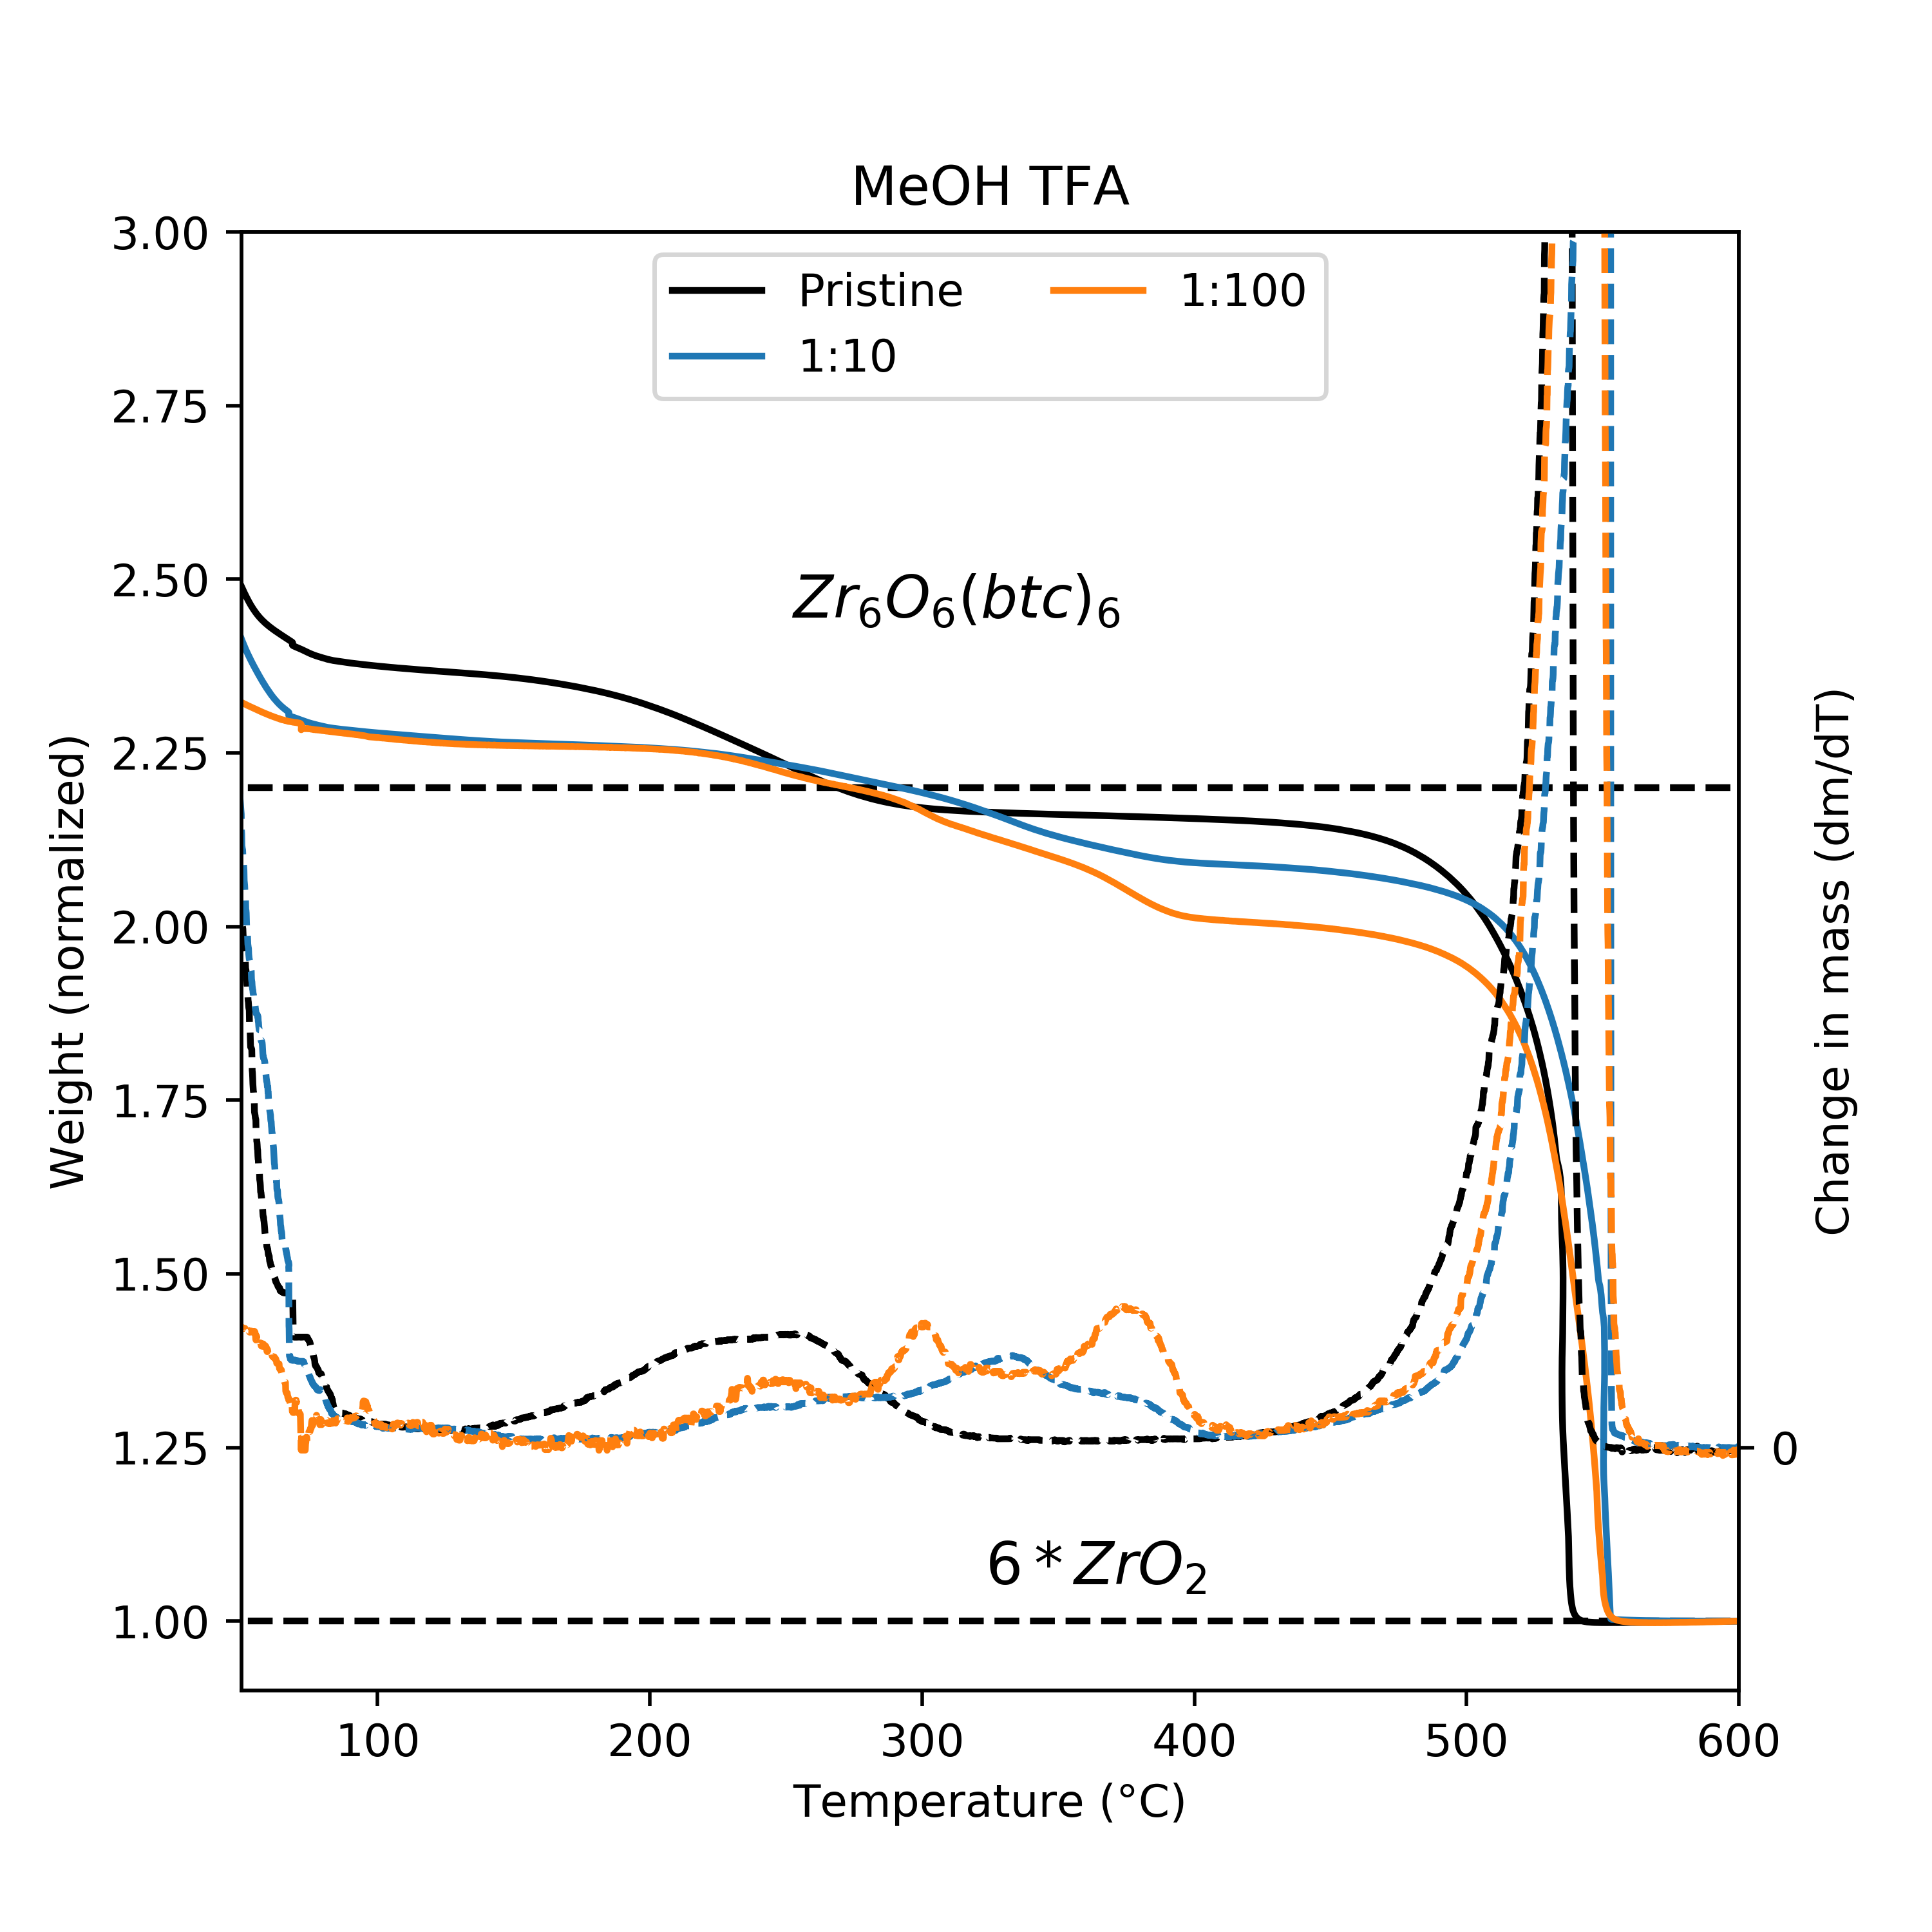
\includegraphics[width=\textwidth]{tga/MeOH-TFA}%
        \label{appx:def:fgr:tga-meoh-tfa}
    \end{subfigure}
    \begin{subfigure}{0.45\linewidth}
        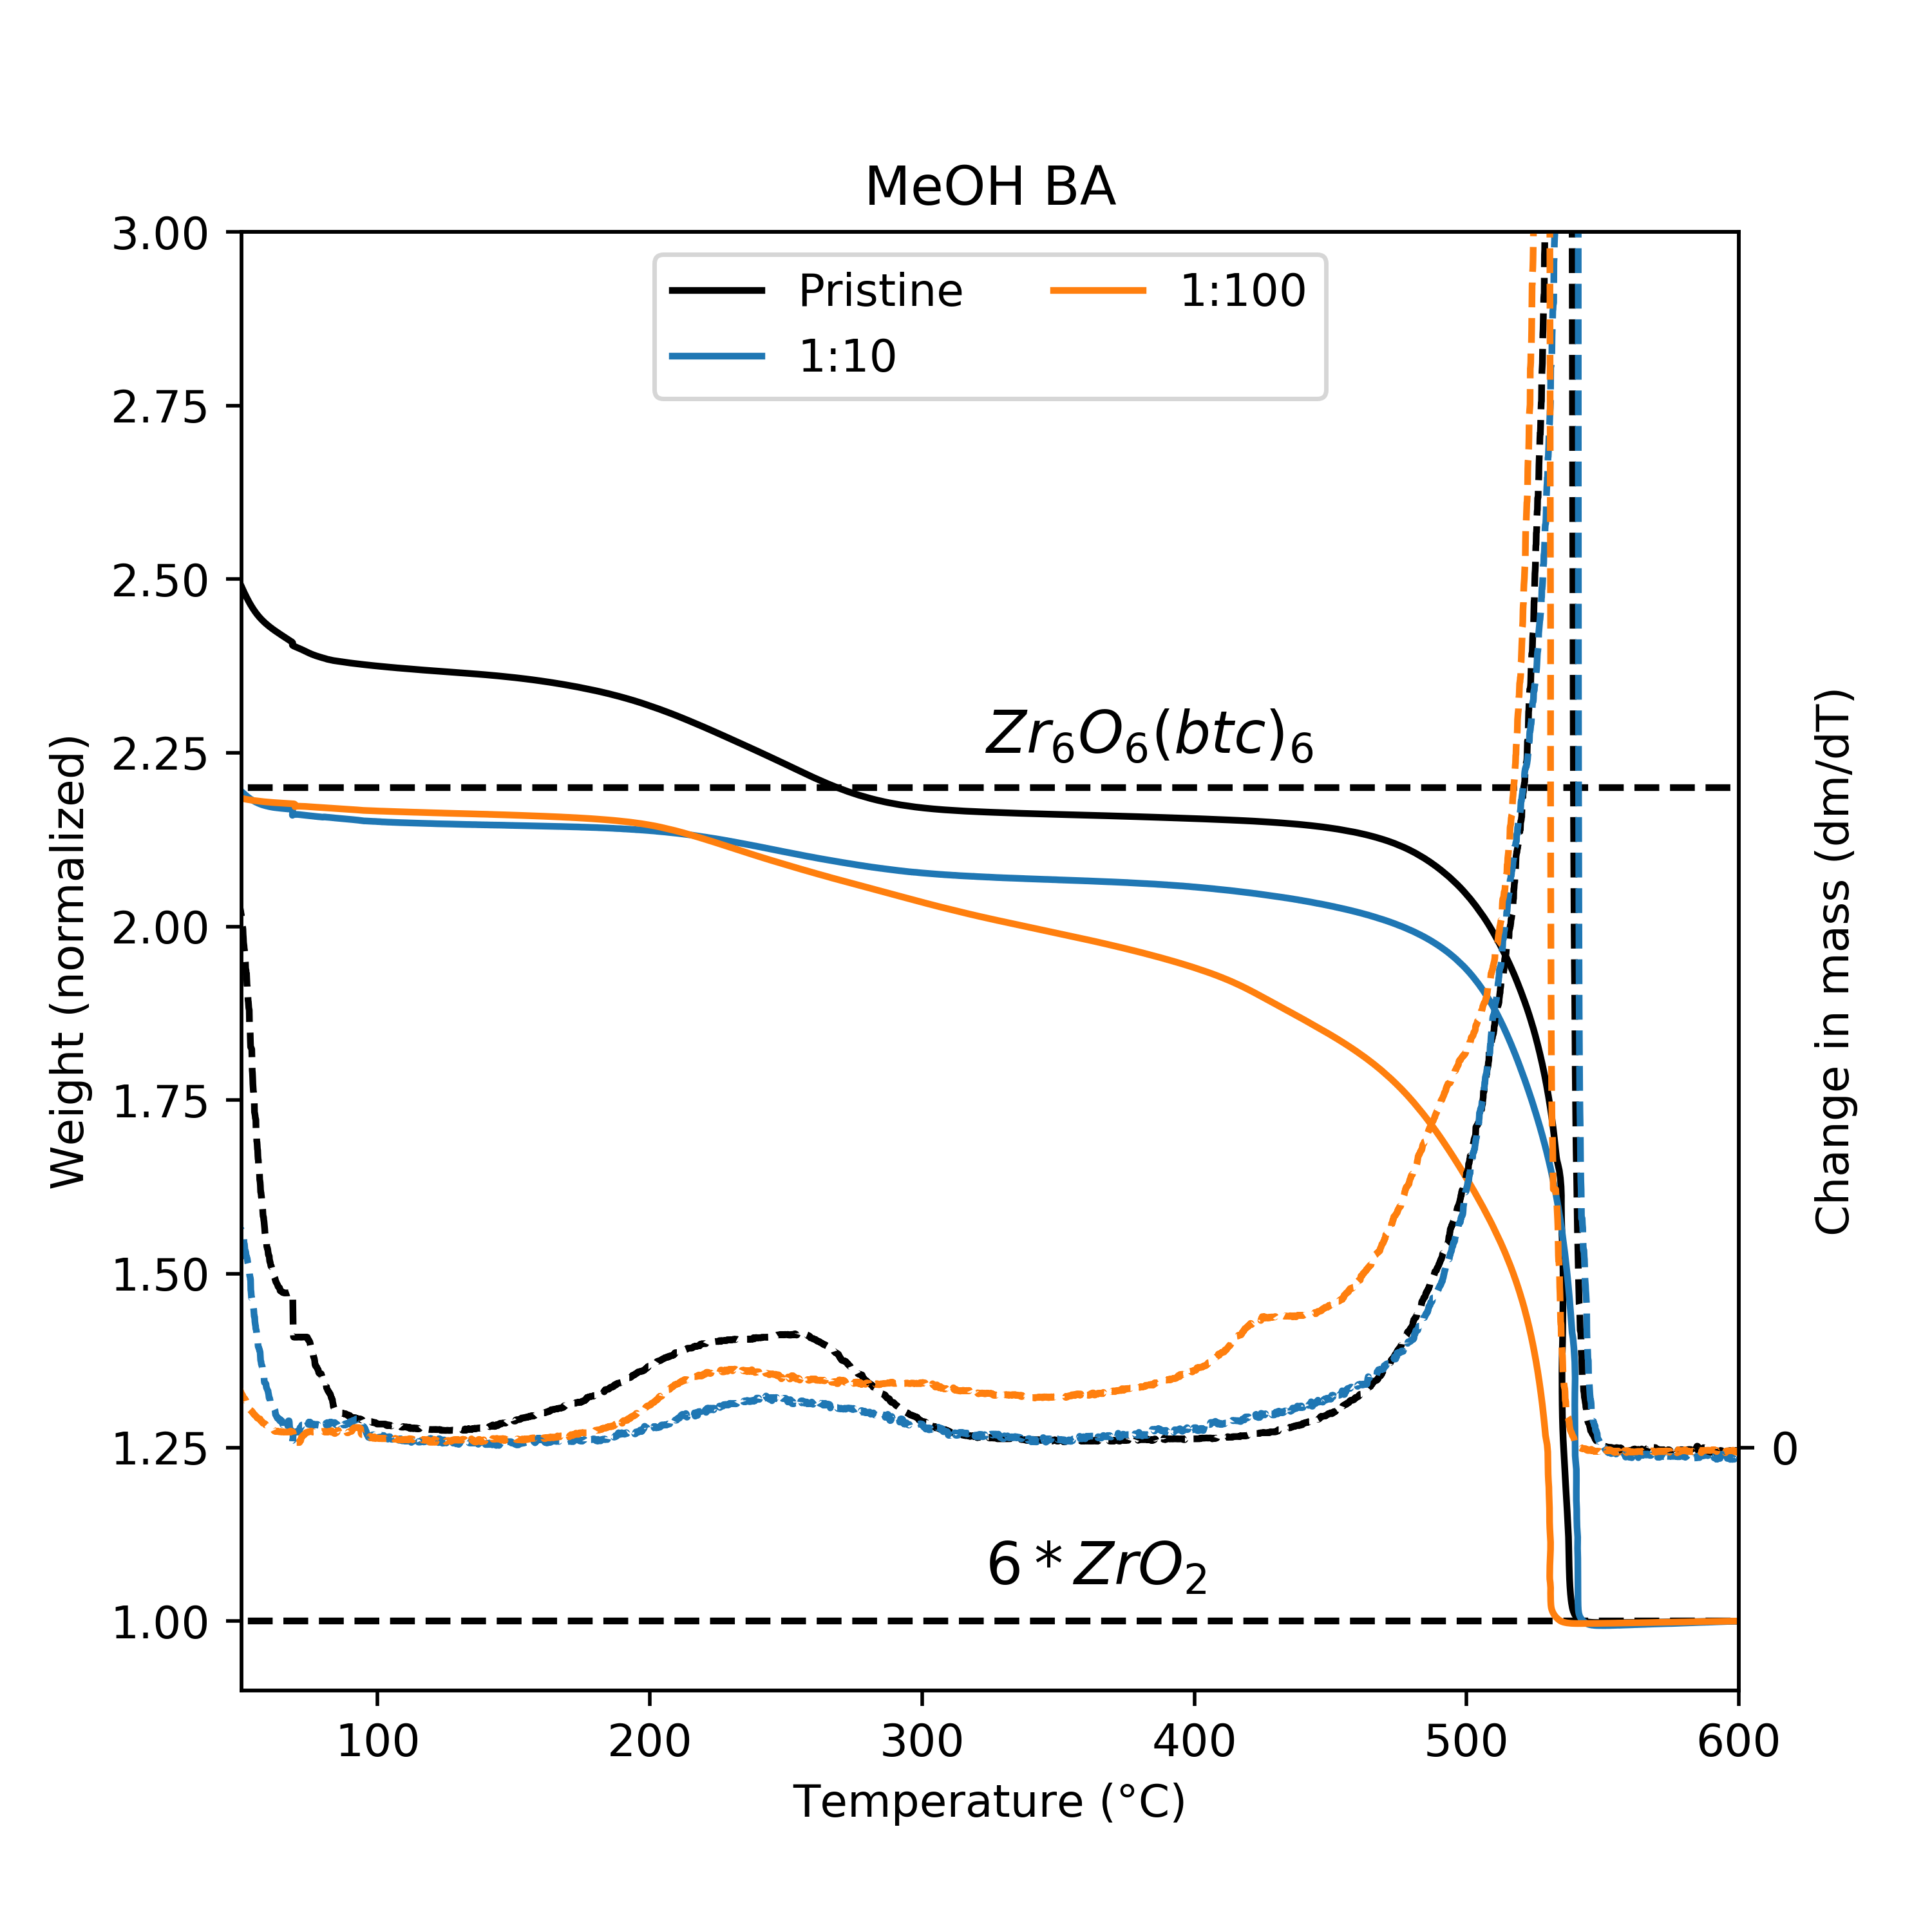
\includegraphics[width=\textwidth]{tga/MeOH-BA}%
        \label{appx:def:fgr:tga-meoh-ba}
    \end{subfigure}

    \caption{TGA curves}%
\end{figure}

\begin{figure}[htb]\ContinuedFloat{}
    \centering

    \begin{subfigure}{0.45\linewidth}
        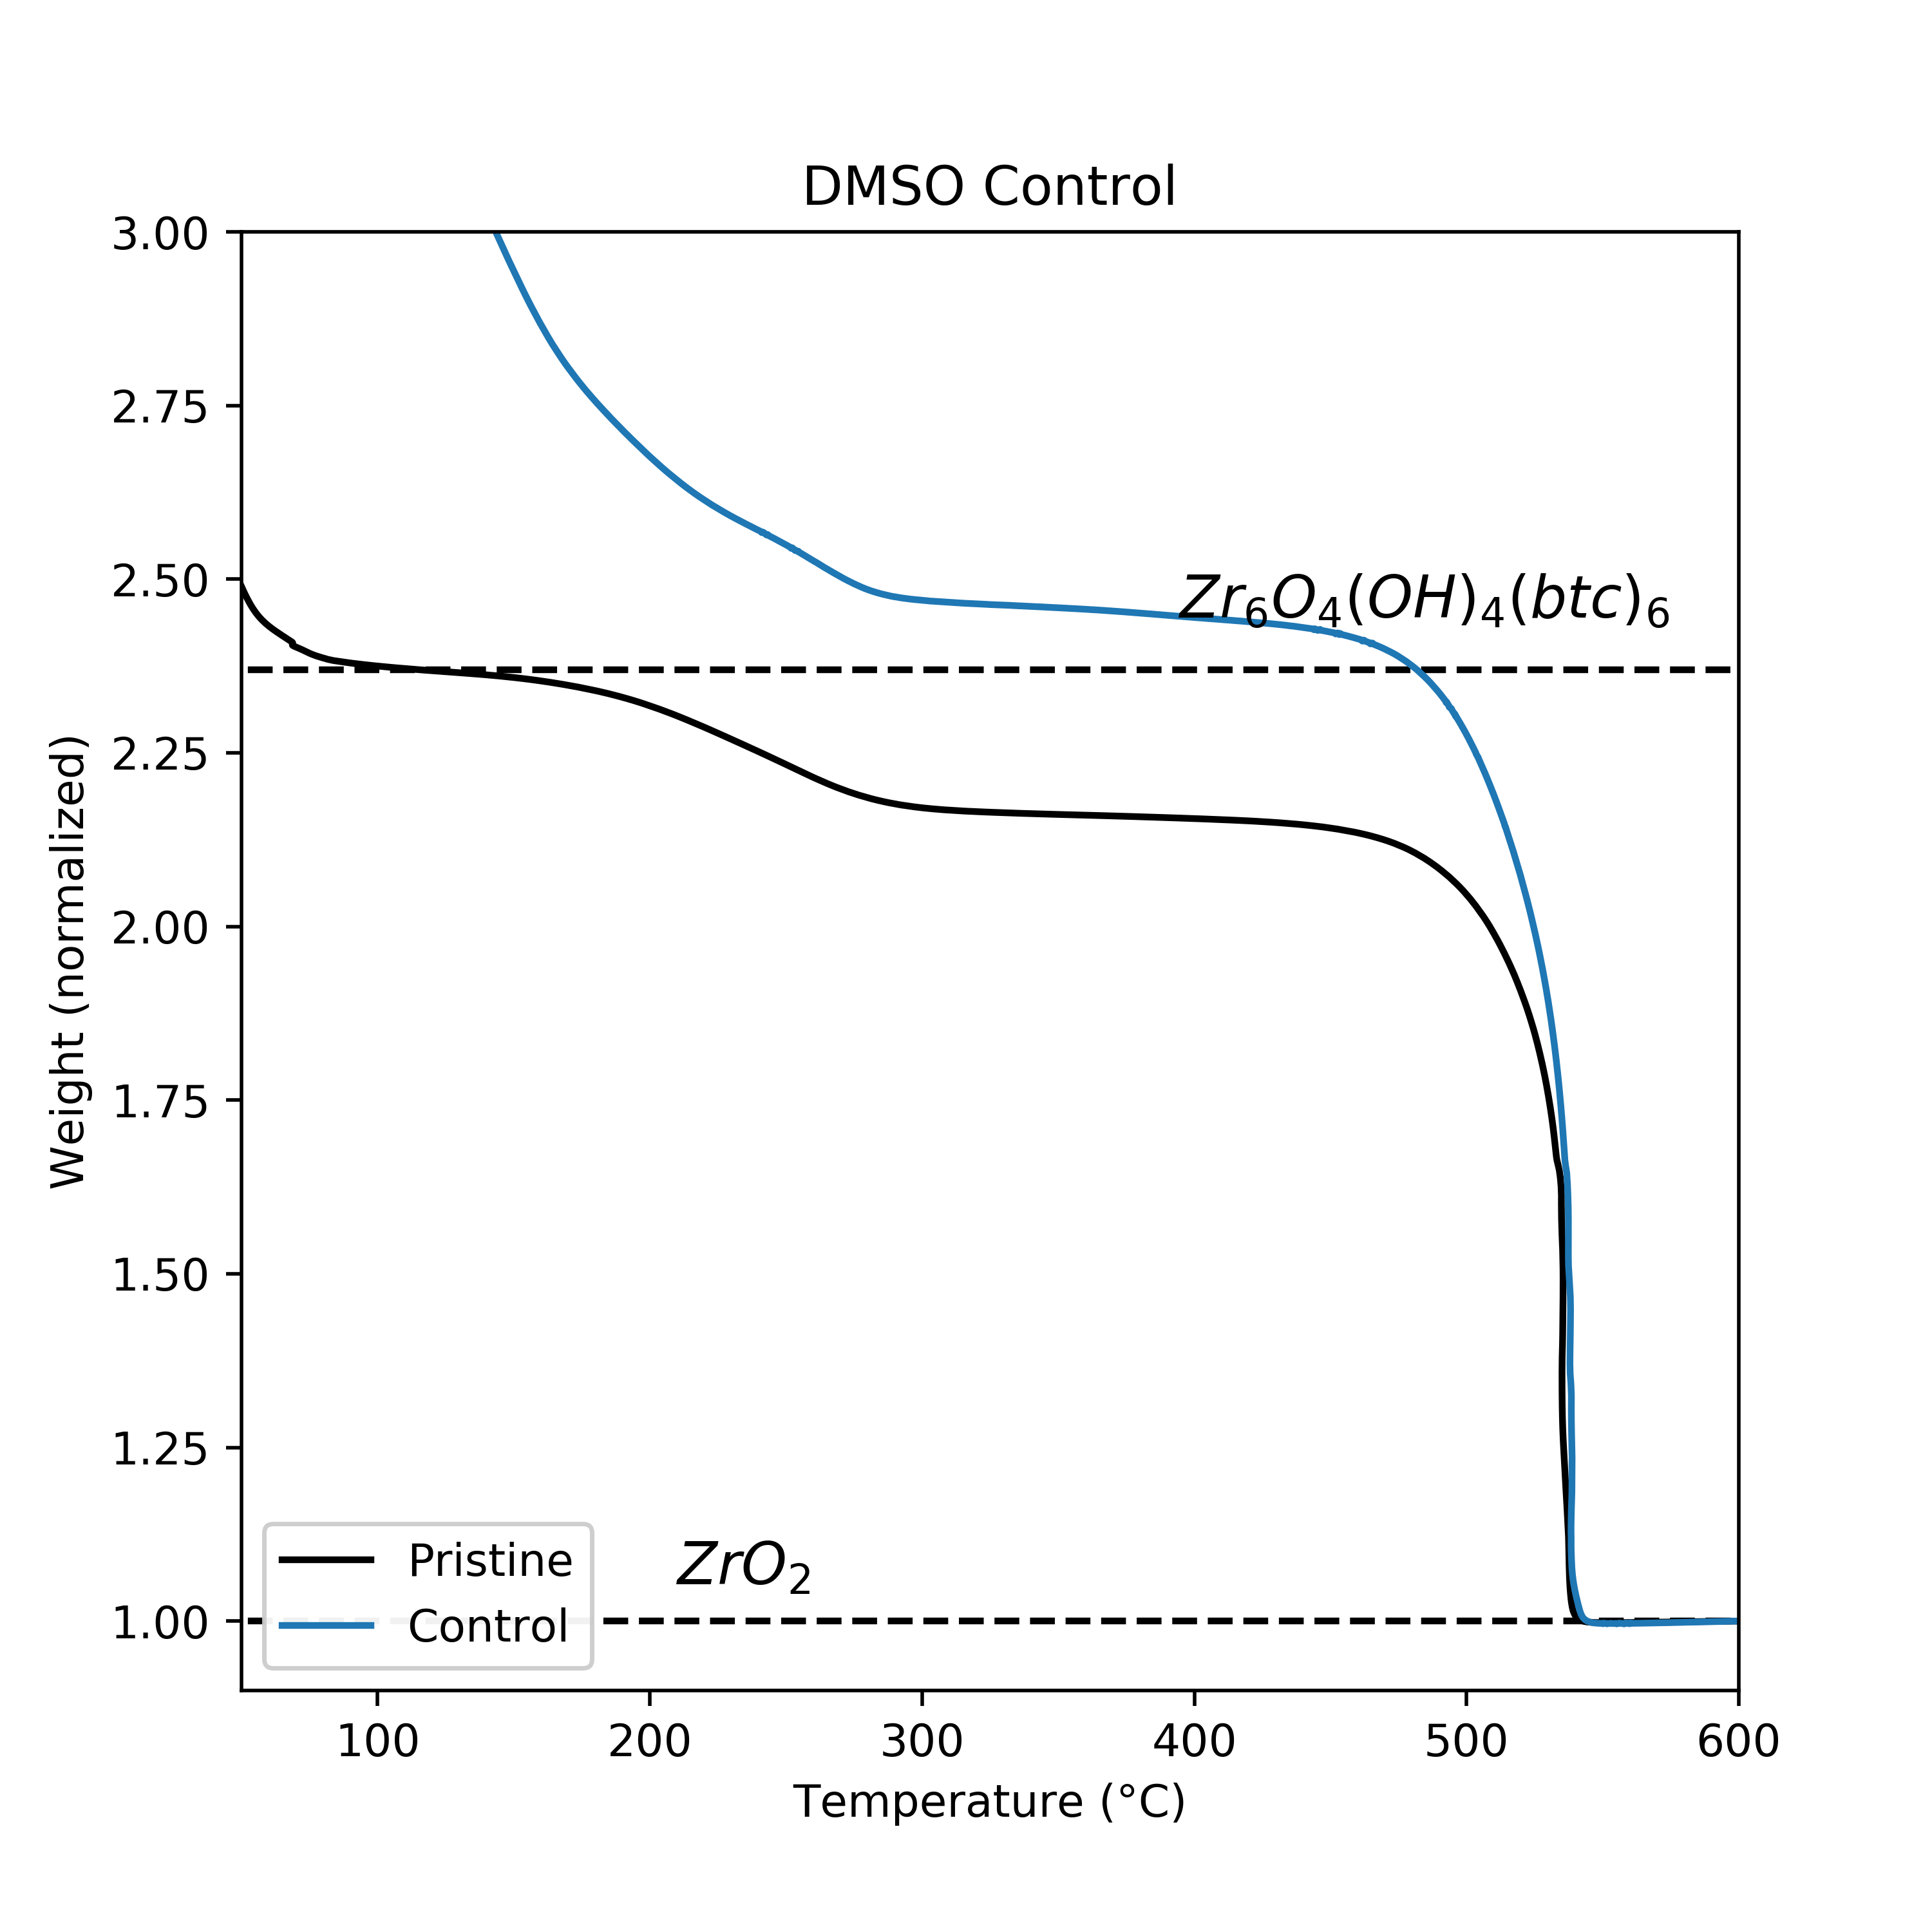
\includegraphics[width=\textwidth]{tga/DMSO-Control}%
        \label{appx:def:fgr:tga-dmso-cont}
    \end{subfigure}

    \begin{subfigure}{0.45\linewidth}
        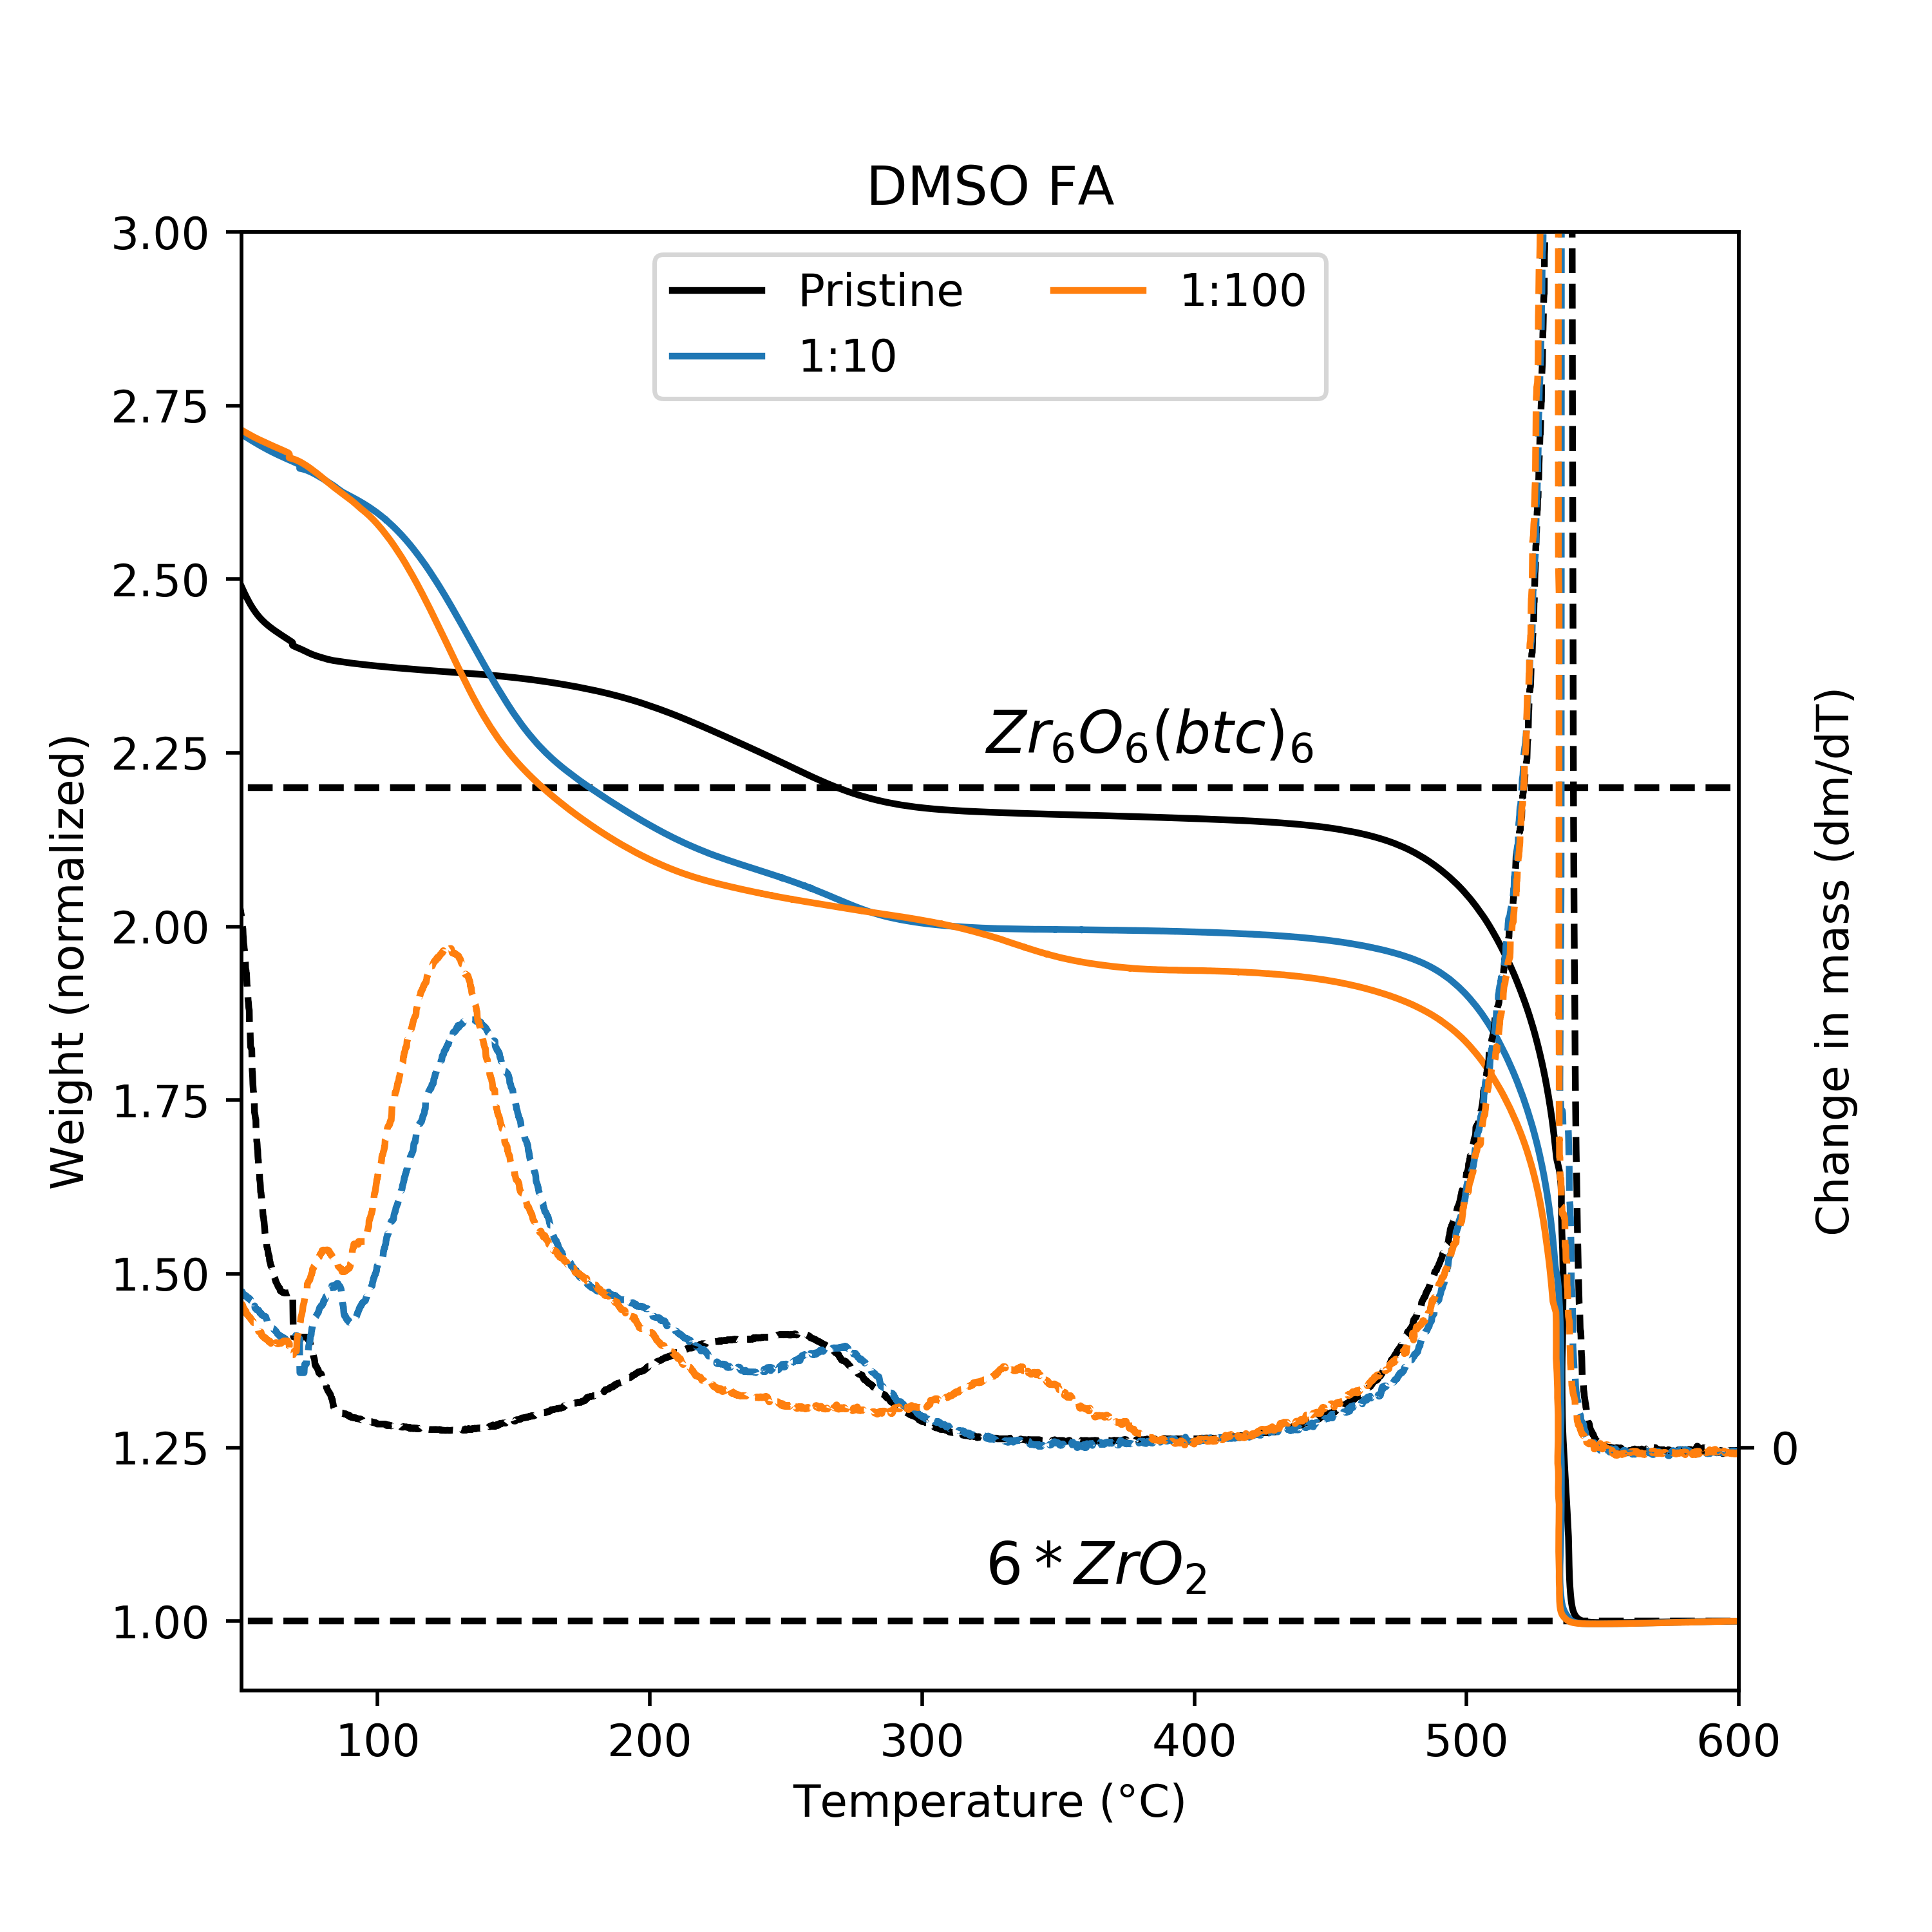
\includegraphics[width=\textwidth]{tga/DMSO-FA}%
        \label{appx:def:fgr:tga-dmso-fa}
    \end{subfigure}
    \begin{subfigure}{0.45\linewidth}
        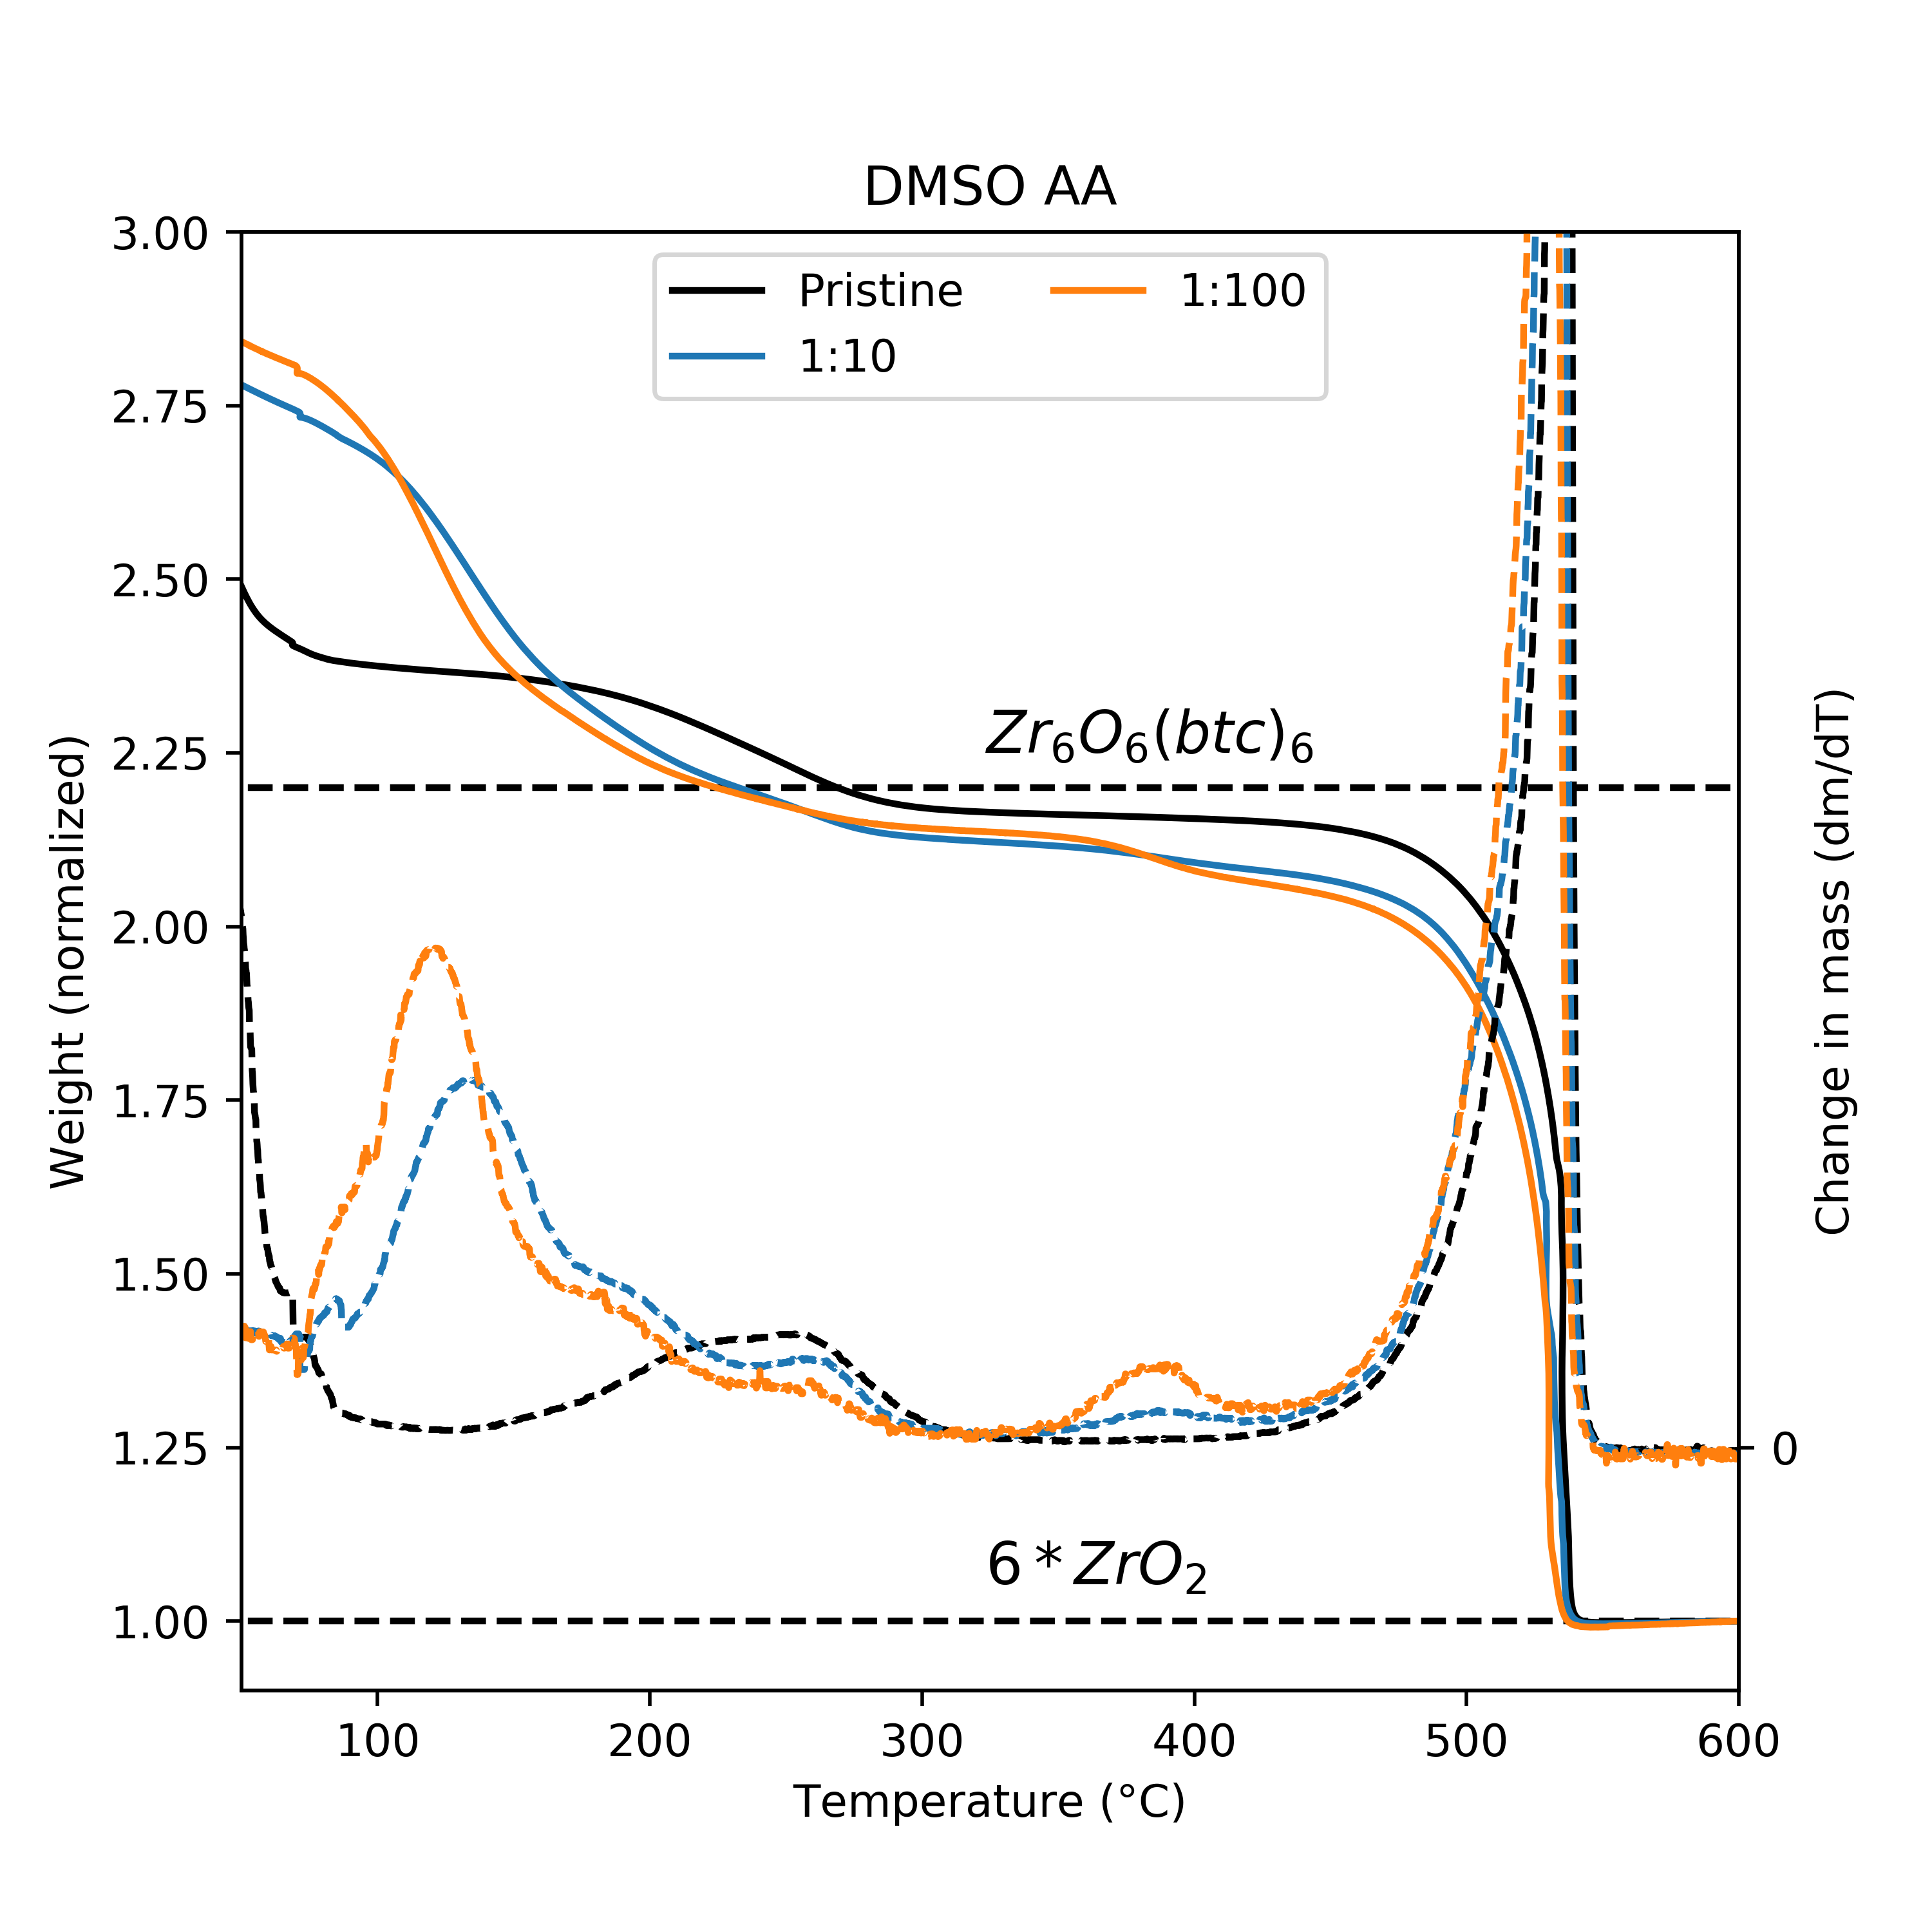
\includegraphics[width=\textwidth]{tga/DMSO-AA}%
        \label{appx:def:fgr:tga-dmso-aa}
    \end{subfigure}

    \begin{subfigure}{0.45\linewidth}
        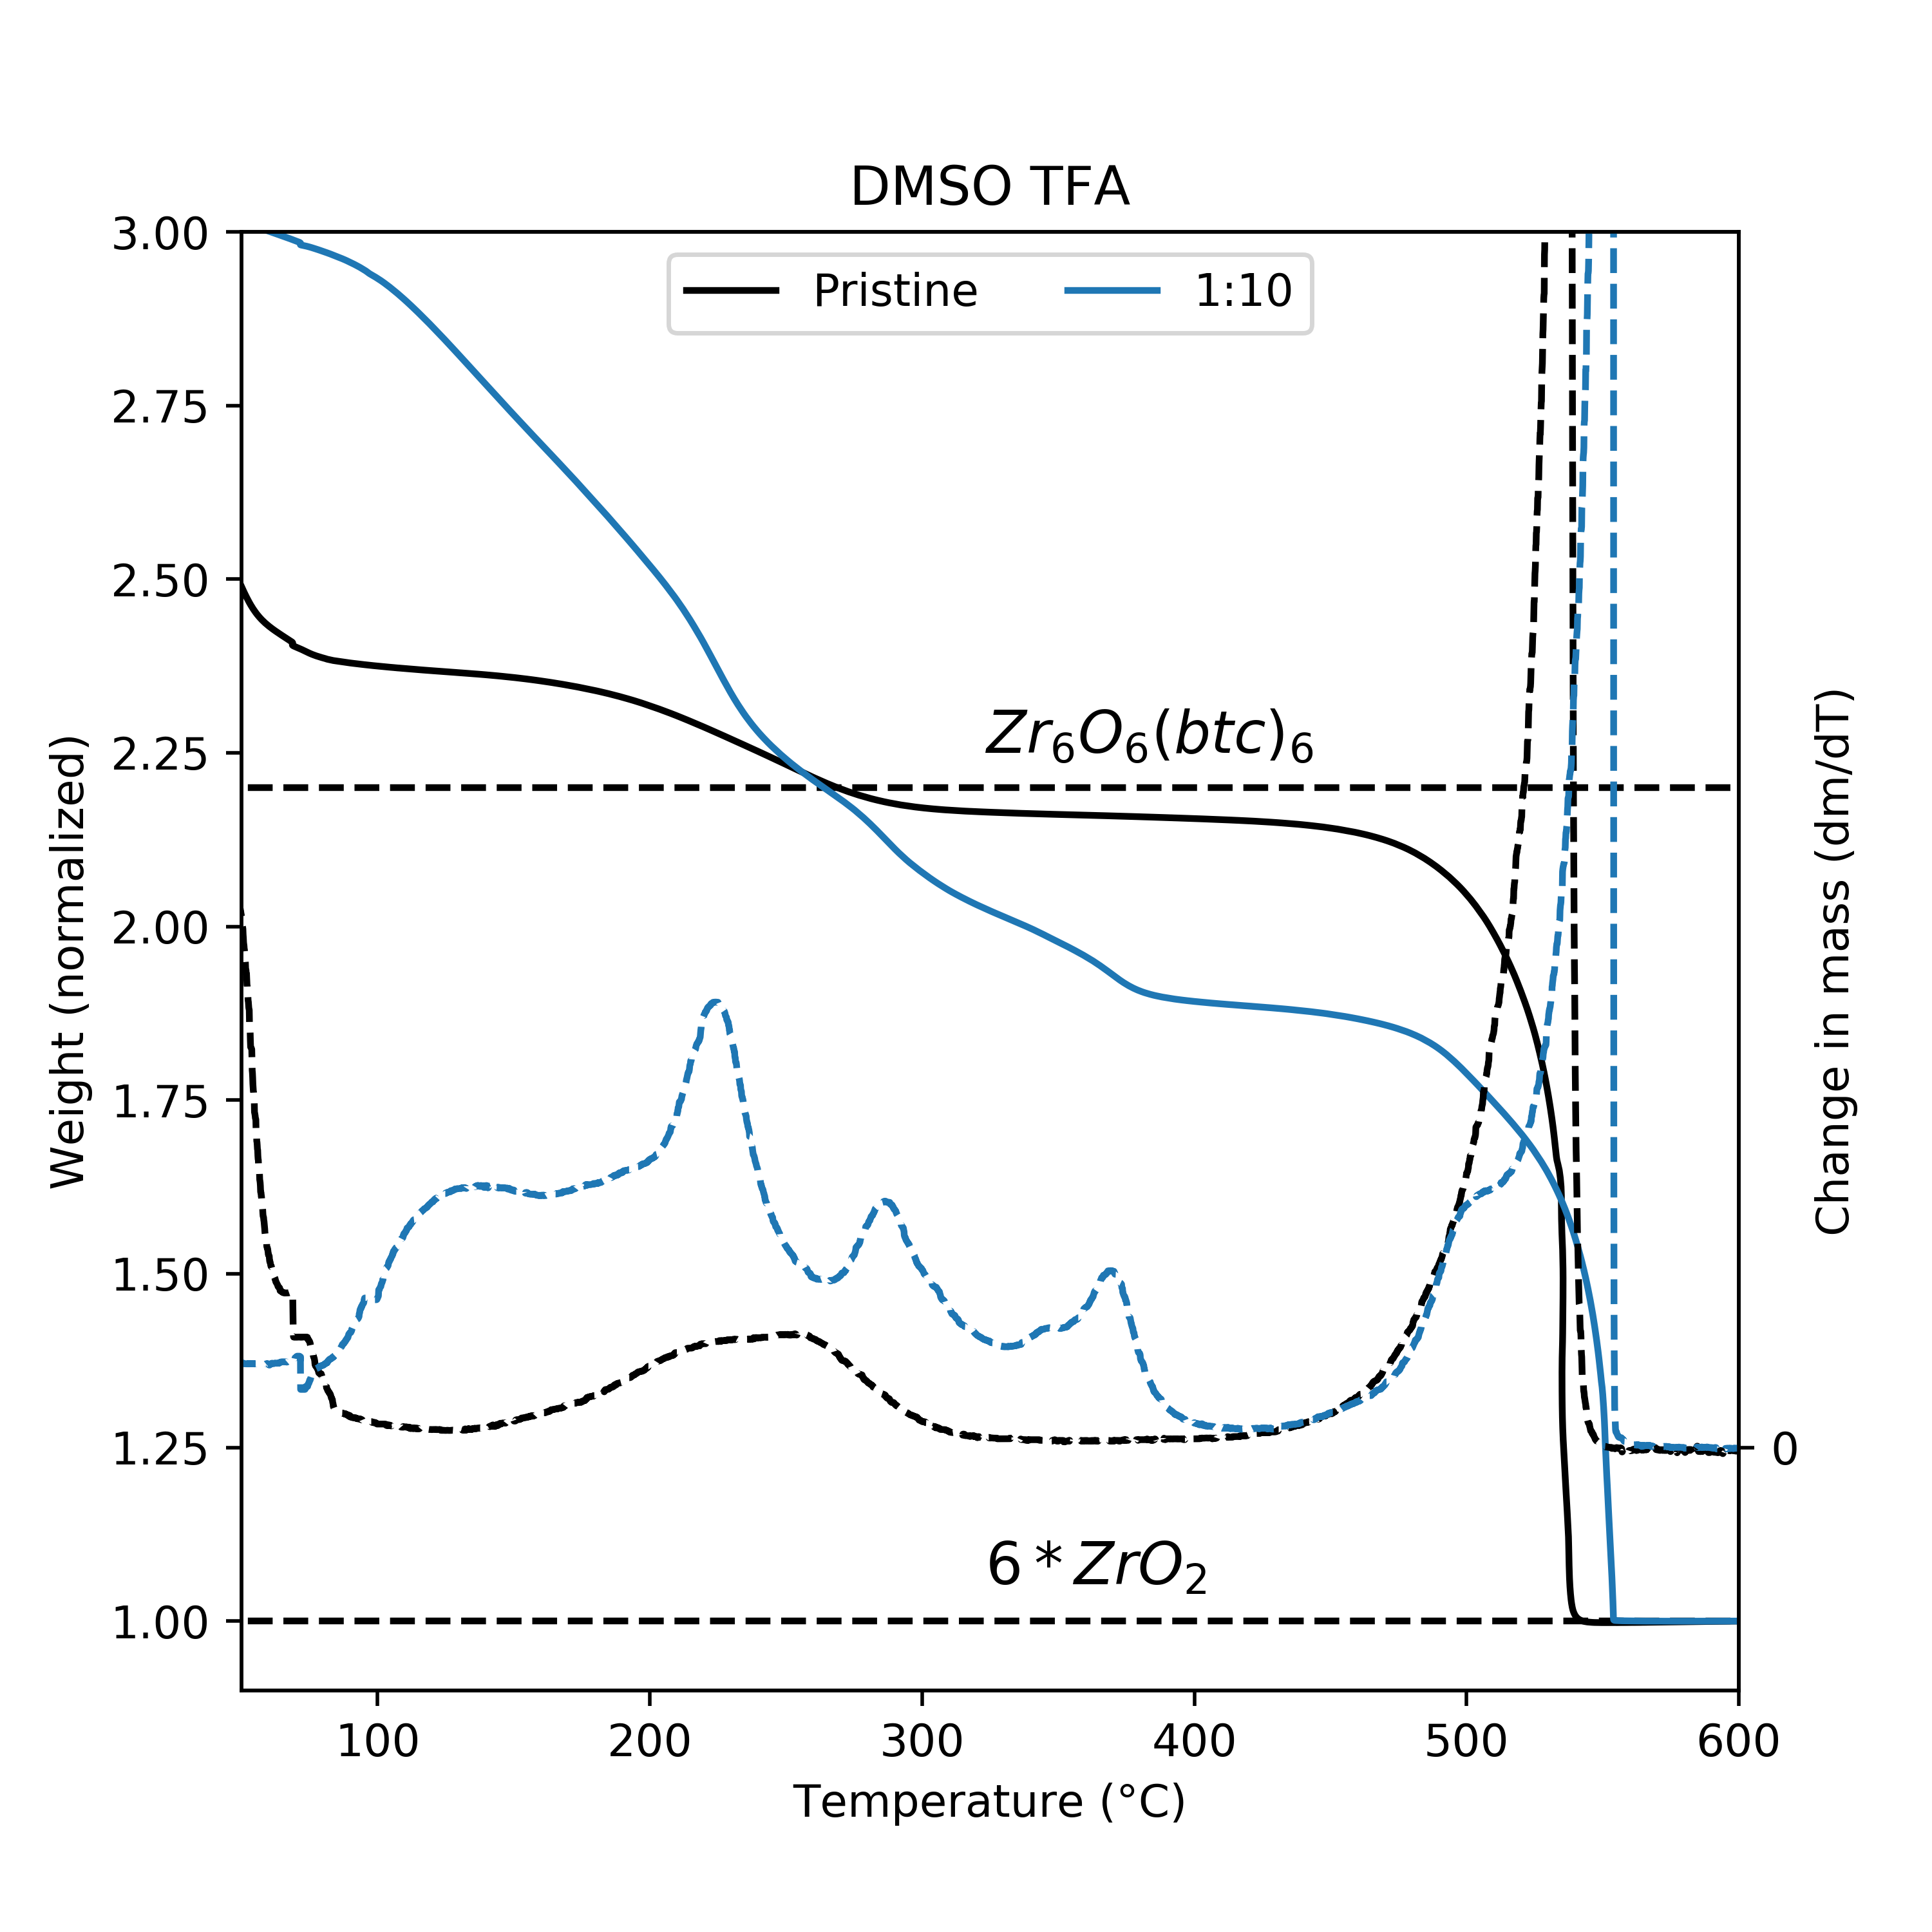
\includegraphics[width=\textwidth]{tga/DMSO-TFA}%
        \label{appx:def:fgr:tga-dmso-tfa}
    \end{subfigure}
    \begin{subfigure}{0.45\linewidth}
        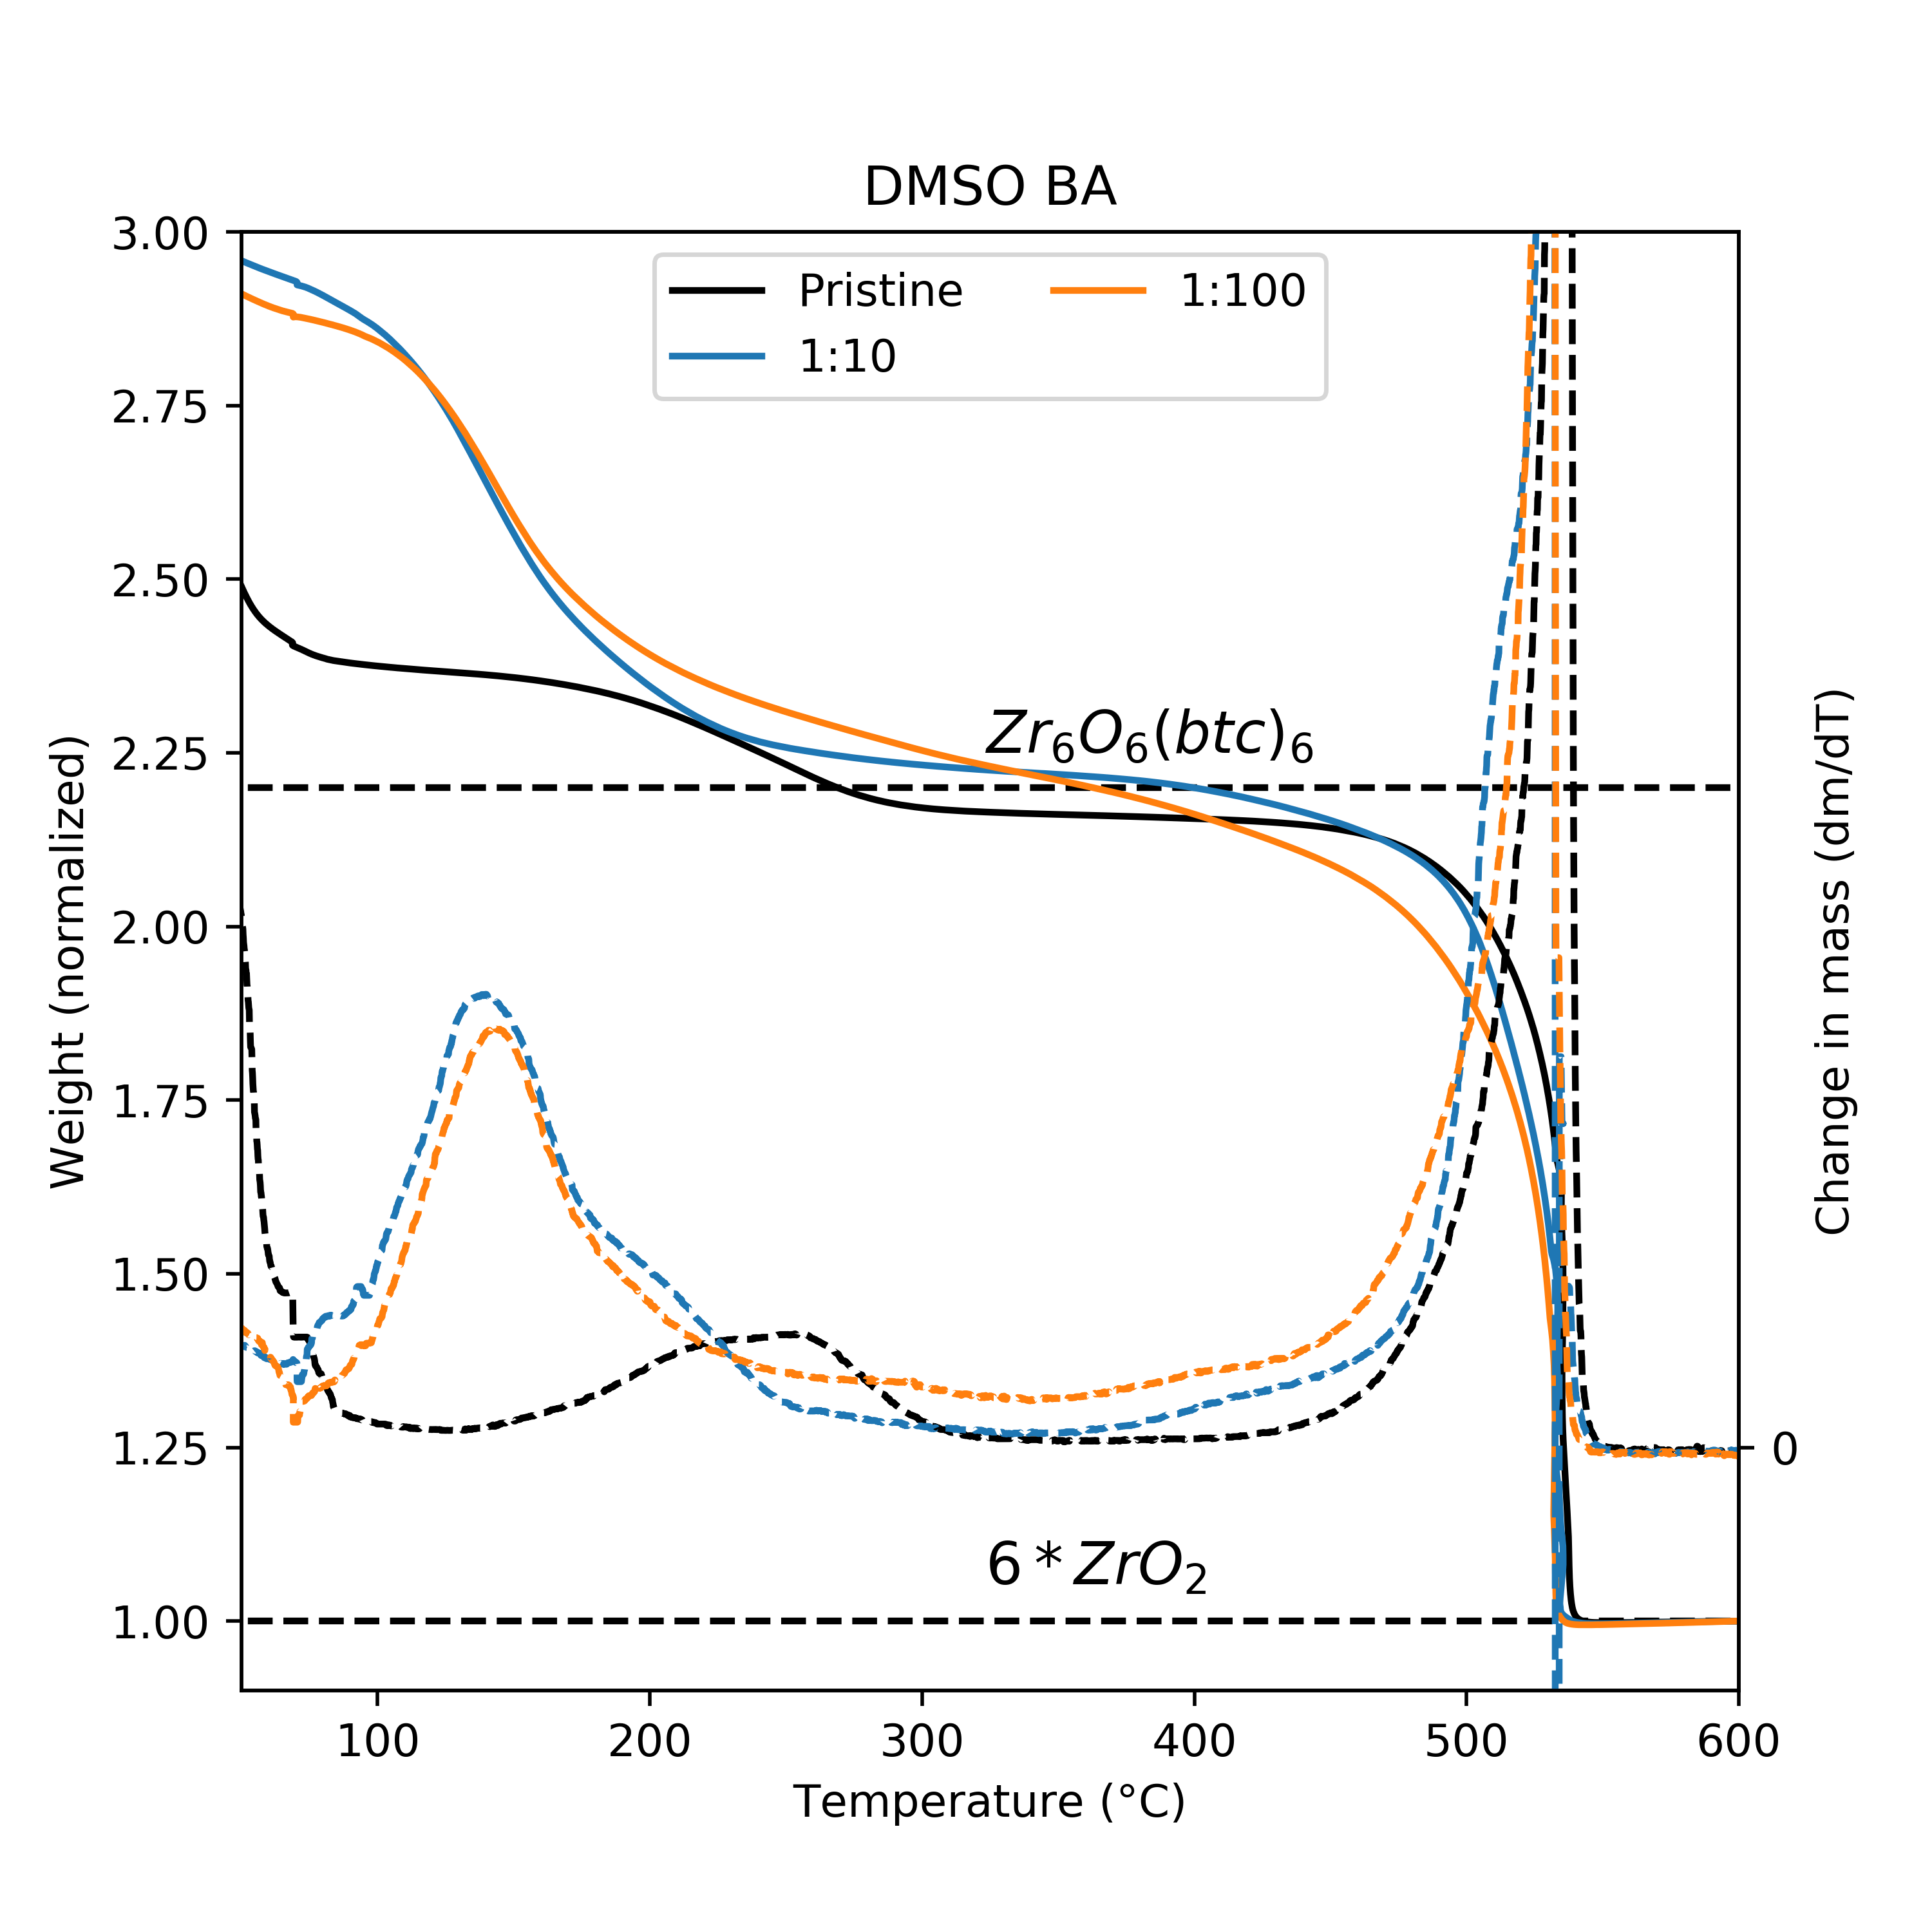
\includegraphics[width=\textwidth]{tga/DMSO-BA}%
        \label{appx:def:fgr:tga-dmso-ba}
    \end{subfigure}

    \caption{TGA curves}%
\end{figure}